\documentclass[ngerman,a4paper,parskip=half]{scrartcl}

\usepackage[ngerman]{babel}
\usepackage[utf8]{inputenc}
\usepackage[onehalfspacing]{setspace}

\usepackage{helvet}
\usepackage[T1]{fontenc} % working hyphenation
\usepackage{lmodern} % better fonts with T1-fontenc
\usepackage{textcomp} % better support of utf8-symbols (adds support of '€')
\usepackage{amsmath, amssymb, amstext}
\usepackage{subcaption}
\usepackage{float}
\usepackage[affil-it]{authblk}
\usepackage[round]{natbib}
\usepackage[nolist]{acronym}
%\usepackage{wrapfig}
%\usepackage[german]{fancyref}
\usepackage{graphicx}
\usepackage{xcolor}
\usepackage{pgfplots}
%\usepackage{eurosym}
\usepackage[export]{adjustbox}

\usepackage[hidelinks]{hyperref}
%\usepackage[left=3.2cm,right=3cm,top=1.7cm,bottom=3cm,includeheadfoot]{geometry}
\usepackage[left=3.2cm,right=3cm,top=2cm,bottom=2.5cm,includeheadfoot]{geometry}

\def \N{\mathbb{N}}
\def \Z{\mathbb{Z}}
\def \Q{\mathbb{Q}}
\def \R{\mathbb{R}}
\def \C{\mathbb{C}}
\def \fov{\mathrm{fov}}

\begin{acronym}[FOV]
	\acro{FOV}{Field of view}
\end{acronym}

\hypersetup{
	pdftitle    = {Streifenlichtprojektion und optische Analyse zur Oberflächeninspektion},
	pdfsubject  = {Streifenlichtprojektion},
	pdfauthor   = {Dennis~Wagner, Johannes~Spangenberg, Leroy~Kramer},
	pdfkeywords = {Streifenlichtprojektion, Humboldt Universität, Informatik, Semesterprojekt},
	%	pdfcreator  = {pdflatex},
	%	pdfproducer = {LaTeX with hyperref},
}

\clubpenalty = 10000 % avoid orphan lines
\widowpenalty = 10000 \displaywidowpenalty = 10000 % avoid widow lines

%Kopf- und Fußzeile
\usepackage{fancyhdr}
\pagestyle{fancy}
\fancyhf{}

%Kopfzeile links bzw. innen
\fancyhead[L]{\nouppercase{\leftmark}}
%Kopfzeile rechts bzw. außen
%\fancyhead[R]{\today}
%Linie oben
\renewcommand{\headrulewidth}{0.5pt}

%Fußzeile mittig
\fancyfoot[C]{\thepage}
%Linie unten
\renewcommand{\footrulewidth}{0.5pt}

\begin{document}

% ---------------------------------------------------------------------------- %

\definecolor{HUblue}{RGB}{0, 55, 108}

\begin{titlepage}
\begin{center}

%\colorbox{HUblue!30}{
\begin{minipage}{\textwidth}
	\begin{minipage}[c]{.8\textwidth}
		\textsc{\LARGE Humboldt-Universität zu Berlin}
		
		Institut für Informatik\\
		Lehrstuhl Signalverarbeitung und Mustererkennung
	\end{minipage}\hfill
	\begin{minipage}[c]{.2\textwidth}
		
\includegraphics{husiegel}
	\end{minipage}
\end{minipage}
%}
\vspace{1.5cm}

\textsc{\Large Semesterprojekt}\\[0.5cm]

% Title
\newcommand{\HRule}{\rule{\linewidth}{0.5mm}}
\HRule \\[0.4cm]
{\huge \bfseries Streifenlichtprojektion und optische Analyse zur Oberflächeninspektion}
\HRule \\[1.5cm]

% Author and supervisor
\begin{minipage}{0.4\textwidth}
\begin{flushleft} \large
\emph{Autoren:}\\
Dennis~Wagner,\\
Johannes~Spangenberg,\\
Leroy~Kramer
\end{flushleft}
\end{minipage}
\hfill
\begin{minipage}{0.4\textwidth}
\begin{flushright} \large
\emph{Betreuende Hochschullehrerin:} \\
Prof.~Dr.~Meffert
\end{flushright}
\end{minipage}

\vfill

% Unterer Teil der Seite
{\large \today}

\end{center}
\end{titlepage}

\tableofcontents
\newpage

% ---------------------------------------------------------------------------- %

\section{Einleitung}
\label{sec:introduction}

In verschiedenen Fällen ist es hilfreich oder notwendig ein \emph{komplexes} dreidimensionales Objekt zu vermessen. Aus solchen Vermessungen resultierende Modelle können beispielsweise in der Unterhaltungsindustrie für die Film- und Spielproduktion verwendet werden. So lassen sich heutzutage dank solcher Verfahren vergleichsweise einfach Personen und Objekte für Spiele modellieren. Außerdem ermöglichen Verfahren zur Vermessung von Oberflächen automatisierte Qualitätskontrollen und neue Methoden zur automatisierten Fertigung oder Verarbeitung.

In diesem Projekt geht es um die \emph{Streifenlichtprojektion}. Dabei wird ein Streifen auf eine Oberfläche projiziert um aus einer Aufnahme der projizierten Linie die Form der Struktur zu rekonstruieren. In diesem Projekt projiziert ein einfacher Linienlaser eine Linie auf eine Struktur. Eine Webcam nimmt diese Struktur samt Linie auf. Mit diesen Bildern können 3-D-Koordinaten von Punkten auf der Laserlinie berechnet werden. Um von einer Struktur mehr Werte zu bekommen, wird dieser Vorgang mit unterschiedlichen Ausrichtungen des Lasers oder mit verschiedenen Positionierungen von dem Aufnahmesetup und der Struktur wiederholt. Schwerpunkt dieses Projektes ist der Test und die Auswertung von unterschiedlichen Verfahren zur Linienerkennung.

Die Arbeit behandelt in Kapitel~\ref{sec:basics} zunächst ein paar wichtige Grundlagen für das Projekt. Dazu gehören \emph{normalisierte Bildkoordinaten}, die \emph{perspektivische Projektion} und die mathematischen Methoden zur Rekonstruktion der Szene. Danach geht es in Kapitel~\ref{sec:realization} um die Umsetzung des Projektes. Dabei wird zunächst die verwendete Hardware betrachtet und der grobe Aufbau der Software beschrieben. Ab Abschnitt~\ref{sec:controller} wird auf verschiedenen Komponenten der Implementierung nochmals genauer eingegangen. In dem Kapitel~\ref{sec:evaluation} geht es um die Auswertung der Ergebnisse worauf in Kapitel~\ref{sec:summary} abschließend noch eine Zusammenfassung folgt.

% ---------------------------------------------------------------------------- %

\section{Theoretische und technische Grundlagen}
\label{sec:basics}

In den letzten Jahrzehnten haben sich zusätzlich zu der hier verwendeten Methode viele verschiedene Techniken entwickelt, mit denen dreidimensionale Strukturen der realen Welt vermessen werden können. So existieren zusätzlich zur Streifenlichtprojektion Verfahren wie \emph{Stereo-Vision}, \emph{Structure from Motion}, \emph{Shape from Shading} und \emph{Time of Flight}. Im Folgenden wird auf wichtige Grundlagen eingegangen, die für das Projekt benötigt werden.

\subsection{Normalisierte Bildkoordinaten}
\label{sec:imagecoordinates}

Ein \emph{digitales Bild} kann als eine zweidimensionalen Matrix dargestellt werden, die für jeden Pixel eine Farbe definiert. Dabei eignen sich die Indizes des Bilder allerdings nur begrenzt zur Beschreibung von Positionen auf dem Bild. Existieren beispielsweise mehrere Inhaltsgleiche Bilder mit unterschiedlicher Abtastrate (Auflösung), so beschreiben die selben Indizes auf jedem Bild eine inhaltlich andere Position. Aus diesem Grund werden in vielen Situationen \emph{normalisierte Bildkoordinaten} verwendet. Das Ziel der normalisierten Bildkoordinaten ist es, Positionen auf einem Bild unabhängig von der Auflösung ausdrücken zu können.

Als normalisierte Bildkoordinaten wird hier ein Tupel aus zwei reellen Zahlen $(u,v)$ verwendet. Dabei ist $v$ aus dem Intervall $[-1,1]$. Der Wertebereich von $u$ ergibt sich entsprechend aus dem Seitenverhältnis $r$: $u \in [-r,r]$. Dabei sollte erwähnt werden, dass normalisierte Bildkoordinaten je nach Anwendungsgebiet auch anders definiert werden können. So kann es je nach Sachverhalt sinnvoll sein, dass für $u$ ebenfalls $u \in [-1,1]$ gilt oder, dass sich $u$ und $v$ im Wertebereich $[0,1]$ befinden.

Um aus den Indizes $(i,j)$ eines Pixels die normalisierten Bildkoordinaten $(u,v)$ zu berechnen, kann hier folgende Gleichung verwendet werden:
\[ \begin{pmatrix}
u \\ v
\end{pmatrix} = 2 \cdot \begin{pmatrix}
\frac{i r}{s_x - 1} \\
\frac{j}{s_y - 1}
\end{pmatrix} - \begin{pmatrix}
r \\ 1
\end{pmatrix} \]
Mit der Bildauflösung $(s_x, s_y)$ und dem Seitenverhältnis $r = s_x/s_y$.

\subsection{Perspektivische Projektion}
\label{sec:perspective}

Bei einer \emph{perspektivischen Projektion} (Abbildung~\ref{fig:perspective}), oder auch \emph{Zentralprojektion}, werden dreidimensionale Punkte auf eine \emph{Bildebene} projiziert. Die Funktion entspricht dabei dem Modell der \emph{Lochkamera} und stellt eine Vereinfachung vieler realen Kameras da. Eine perspektivische Projektion wird durch den Augpunkt $O$ und die Bildebene definiert. Um einen Objektpunkt $X$ auf einen Punkt $X'$ in die Bildebene zu projizieren, wird der Schnittpunkt des \emph{Projektionsstrahls} durch $X$ und $O$ mit der Bildebene bestimmt. Der projizierte Punkt $X'$ wird auch \emph{Bildpunkt} genannt. Die Bildebene wird oft durch eine Blickrichtung der \emph{Kamera} und eine \emph{Brennweite} $f$ definiert. Die Blickrichtung der Kamera entspricht dabei der Normalen der Bildebenen und $f$ ist die Entfernung der Bildebene vom Augpunkt in Blickrichtung.

\begin{figure}
	\centering
	\begin{subfigure}{0.4\textwidth}
		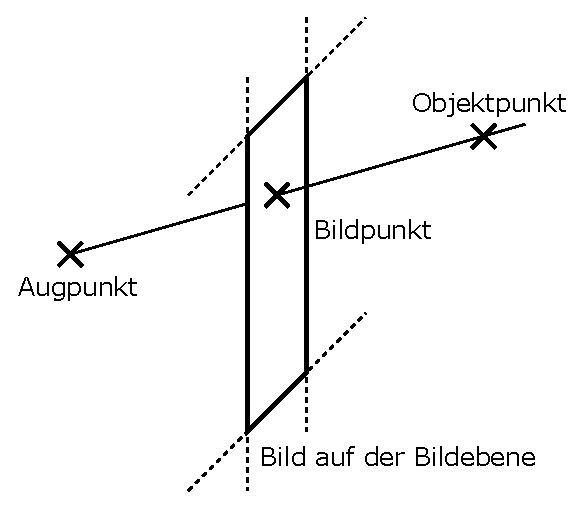
\includegraphics[width=\textwidth]{includes/perspective}
	\end{subfigure}
	\hfill
	\begin{subfigure}{0.4\textwidth}
		
\includegraphics[width=\textwidth]{includes/perspective2}
	\end{subfigure}
	\caption{Perspektivische Projektion}
	\label{fig:perspective}
\end{figure}

Oft wird die perspektivische Projektion in Verbindung mit Bildern, wie sie in Abschnitt~\ref{sec:imagecoordinates} beschrieben werden, verwendet und nicht mit konkreten Bildpunkten. Dazu muss definiert werden, wo sich das Bild auf der Bildebene befindet. Eine offensichtliche Möglichkeit ist die Angabe der Höhe und Breite des Bildes auf der Bildebene, unter der Annahme, dass der am nächsten liegende Punkt der Bildebene zum Augpunkt in der Mitte des Bildes liegt. Wenn das Seitenverhältnis des Bildes beibehalten wird, reicht auch die Angabe der Höhe. Meistens ist es nicht relevant, wo sich die Bildebene genau befindet, sofern jedem Punkt eine Projektionsgerade zugeordnet wird, daher kann die Brennweite nach belieben verändert werden, solange auch die Bildhöhe entsprechend angepasst wird. Aus diesem Grund reicht es oft, nur die Brennweite als Parameter für die Projektion zu nutzen, sofern die Bildhöhe zuvor fest definiert wurde.

Angenommen das Bild ist zwei Einheiten hoch, der Augpunkt ist $O(0,0,0)$ und die Kamera schaut in Richtung der negativen $z$-Achse. Dann kann aus den normalisierten Bildkoordinaten $(u,v)$ der entsprechende Bildpunkt $X'$ ganz einfach über die folgende Gleichung bestimmt werden:
\[ \vec{x'} = \begin{pmatrix}
u \\ v \\ -f
\end{pmatrix} \]

Alternativ zur Brennweite und Bildhöhe wird auch oft das vertikale \ac{FOV} benutzt, um die Projektion zu definieren. Das vertikale \ac{FOV} ist der Winkel zwischen den obersten und untersten Projektionsgeraden des Bildes. Die Brennweite $f$, die Bildhöhe $g$ und das vertikale \ac{FOV} $\fov$ stehen dabei in der folgende Beziehung:
\begin{align*}
	\fov = 2 \cdot \arctan \left( \frac{g}{2 f} \right)
	\Leftrightarrow f = \frac{g}{2 \tan\left(\frac{\fov}{2}\right)}
\end{align*}

\subsection{Triangulation}

Das Prinzip der Triangulation ist es aus zwei Eckpunkten und den Innenwickeln eines Dreiecks den dritten Eckpunkt zu bestimmen. Hier wird der Objektpunkt auf der Laserlinie auf Basis eines Bildpunktes und der Laserausrichtung bestimmt.

\subsubsection{Modell und gegebene Werte}

\begin{figure}
	\centering
	\begin{subfigure}{0.55\textwidth}
		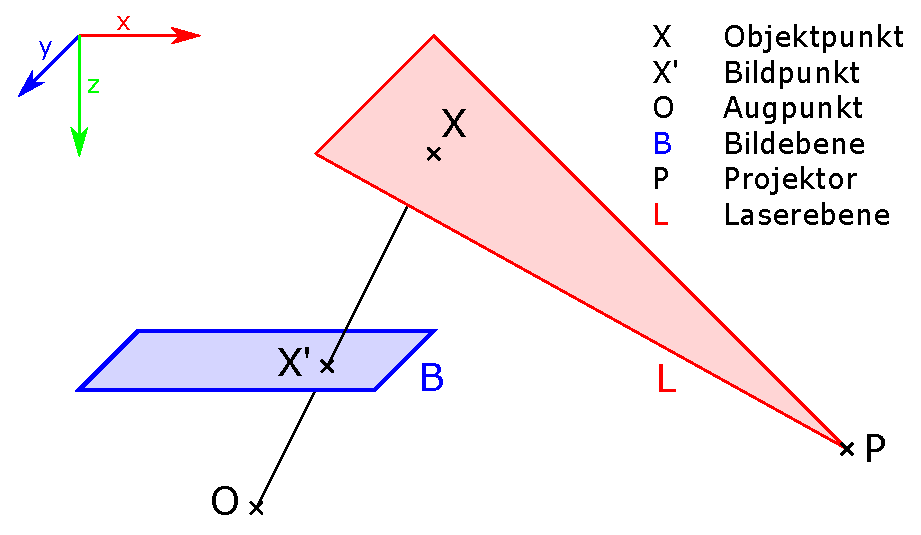
\includegraphics[width=\textwidth]{includes/triangulation3d}
		\caption{dreidimensionales Modell}
		\label{fig:triangulation3d}
	\end{subfigure}
	\hfill
	\begin{subfigure}{0.35\textwidth}
		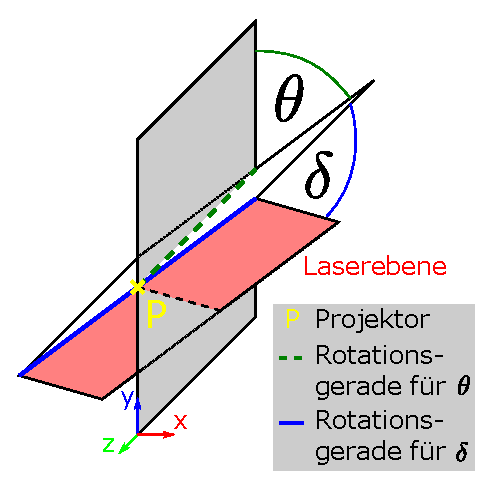
\includegraphics[width=\textwidth]{includes/triangulation_skew_pitch}
		\caption{Ausrichtung der Laserebene L}
		\label{fig:triangulation_skew_pitch}
	\end{subfigure}

	\begin{subfigure}{0.45\textwidth}
		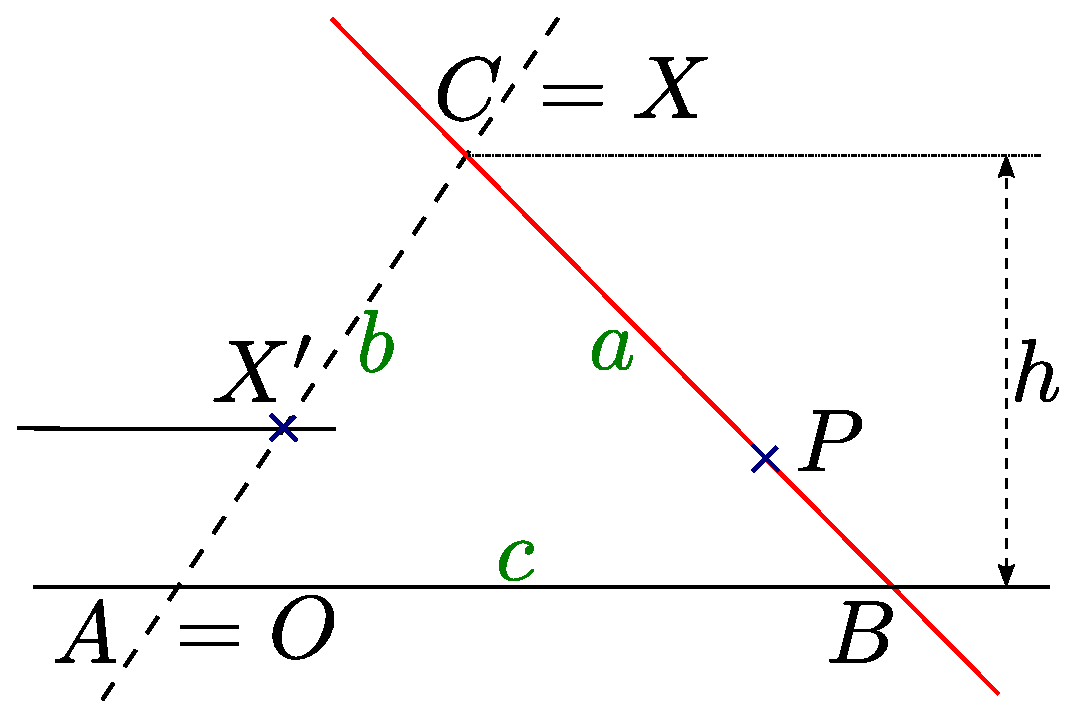
\includegraphics[width=\textwidth]{includes/triangulation2d}
		\caption{vereinfachtes zweidimensionales Modell}
		\label{fig:triangulation2d}
	\end{subfigure}
	\caption{Modell des Setups}
\end{figure}

Als Modell für die Triangulation wird die Abstraktion, wie sie auf Abbildung~\ref{fig:triangulation3d} zu sehen ist, verwendet. Es existiert eine perspektivischen Projektion eines Objektpunktes $X$ auf eine Bildebene $B$, wobei die Blickrichtung entlang der negativen $z$-Achse verläuft. Der Augpunkt $O$ liegt dabei im Koordinatenursprung. Der Bildpunkt wird mit $X'$ bezeichnet. Das projizierte Licht wird durch eine Ebene $L$ dargestellt, die die Position des Projektors, das heißt den Projektionspunkt $P$, und den Objektpunkt $X$ schneidet.

Die durch das Setup gegebenen Werte:

\begin{tabular}{lp{12cm}}
	$P$                &
		Position des Linienprojektors\\[0.5em]
	$f$                &
		Brennweite\\[0.5em]
	$\theta$,$\delta$  &
		Winkel zur Ausrichtung der Ebene $L$. Die Ausgangslage der Ebene ist parallel zur $y$-$z$-Ebene. Die Ebene wird zunächst mit dem Winkel $\theta$ um den Vektor $(0,0,-1)^T$  im mathematisch positiven Drehsinn gedreht. Danach mit dem Winkel $\delta$ um den Vektor $(-\sin(\theta), -\cos(\theta), 0)^T$. Siehe auch Abbildung~\ref{fig:triangulation_skew_pitch}.
\end{tabular}

Zudem ist der Bildpunkt durch normalisierte Bildkoordinaten $(u, v)$ gegeben. Die Brennweite $f$ ist auf eine Bildhöhe von zwei Einheiten angepasst. Damit gilt wie in Abschnitt~\ref{sec:perspective} beschrieben $X'(u, v, -f)$.

\subsubsection{Bestimmung der Entfernung}

Als \emph{Entfernung des Objektpunktes} $h$ wird die negierte 3. Koordinate von $X$ bezeichnet.

Um diese Entfernung zu bestimmen, wird das geometrische Modell des Setups vereinfacht. Als erstes wird ein Basiswechsel auf die Orthogonalbasis
\[ \left\lbrace \begin{pmatrix}
\cos(\theta) \\ \sin(\theta) \\ 0
\end{pmatrix}, \begin{pmatrix}
0 \\ 0 \\ -1
\end{pmatrix}, \begin{pmatrix}
\sin(\theta) \\ \cos(\theta) \\ 0
\end{pmatrix} \right\rbrace \]
vorgenommen, um im folgenden nur die ersten beiden Dimensionen zu betrachten. Der konstruierte zweidimensionale Raum hat die besondere Eigenschaft, dass von der Ebene $L$ und der $x$-$y$-Ebene nur die Geraden $a$ und $c$ übrig bleiben. Eine weitere besondere Eigenschaft ist, dass der Abstand zwischen $X$ und der $x$-$y$-Ebene direkt von einen in den anderen Raum übernommen werden kann. So entspricht $h$ im vereinfachten Modell der 2. Koordinate von $X$. Ein beliebiger Vektor $(v_1, v_2, v_3)^T$ im dreidimensionalen Model entspricht im zweidimensionalen Modell dem Vektor $(\cos(\theta) \cdot v_1 - \sin(\theta) \cdot v_2, -v_3)^T$.

Die Geraden $a$ und $c$ bilden zusammen mit der Geraden $b$, welche durch die Punkte $O$, $X$ und $X'$ verläuft, ein Dreieck, dessen Eckpunkte $A=O$, $B$ und $C = X$ sind. Dies ist auch nochmal in Abbildung~\ref{fig:triangulation2d} zu sehen. Angenommen die Koordinaten von $P$ und $X'$ in der zweidimensionalen Darstellung sind $(p_1,p_2)$ und $(x'_1, x'_2)$, so können die Winkel $\alpha$ und $\beta$ und die Länge der Strecke zwischen $A$ und $B$ wie folgt berechnet werden:
\begin{align*}
	\alpha &= \frac{\pi}{2} - \arctan\left(\frac{x'_1}{x'_2}\right)\\
	\beta &= \frac{\pi}{2} + \delta\\
	\overline{AB} &= p_1 + \tan(\delta) \cdot p_2
\end{align*}

Die Entfernung $h$ ergibt sich daraufhin aus der folgenden Gleichung:
\[ h = \frac{\overline{AB} \cdot \sin(\alpha) \cdot \sin(\beta)}{\sin(\pi - \beta - \alpha)} \]

\subsubsection{Bestimmung der Koordinaten}

Nachdem die Entfernung $h$ des Objektpunktes bekannt ist, kann der Objektpunkt $X$ aus dem Bildpunkt bestimmt werden:
\[ \vec{x} = \frac{h}{f} \cdot \vec{x'} = \frac{h}{f} \cdot \begin{pmatrix}
u \\ v \\ -f
\end{pmatrix} \]

% ---------------------------------------------------------------------------- %

\section{Aufbau und Algorithmen}
\label{sec:realization}

\subsection{Hardware}

Die Hardware besteht aus einer Webcam und einem günstigen Linienlaser, der auf einem Modellbauservo montiert ist. Laser und Servo werden von einem Mikrocontroller gesteuert, welcher wiederum über USB mit der Software kommuniziert. Der Aufbau ist in der Abbildung~\ref{fig:hardware} zu sehen.

\begin{figure}
	\centering
	\begin{subfigure}{0.45\textwidth}
		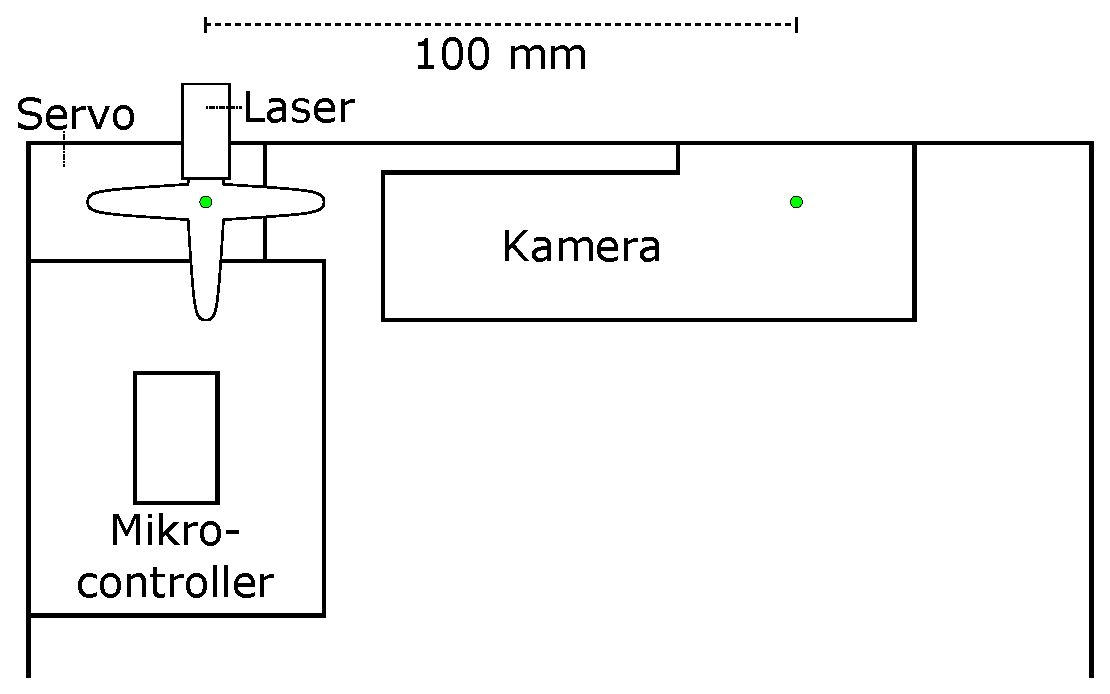
\includegraphics[height=4.5cm]{includes/hardware_schematic}
		\caption{schematische Darstellung}
	\end{subfigure}
	\hfill
	\begin{subfigure}{0.4\textwidth}
		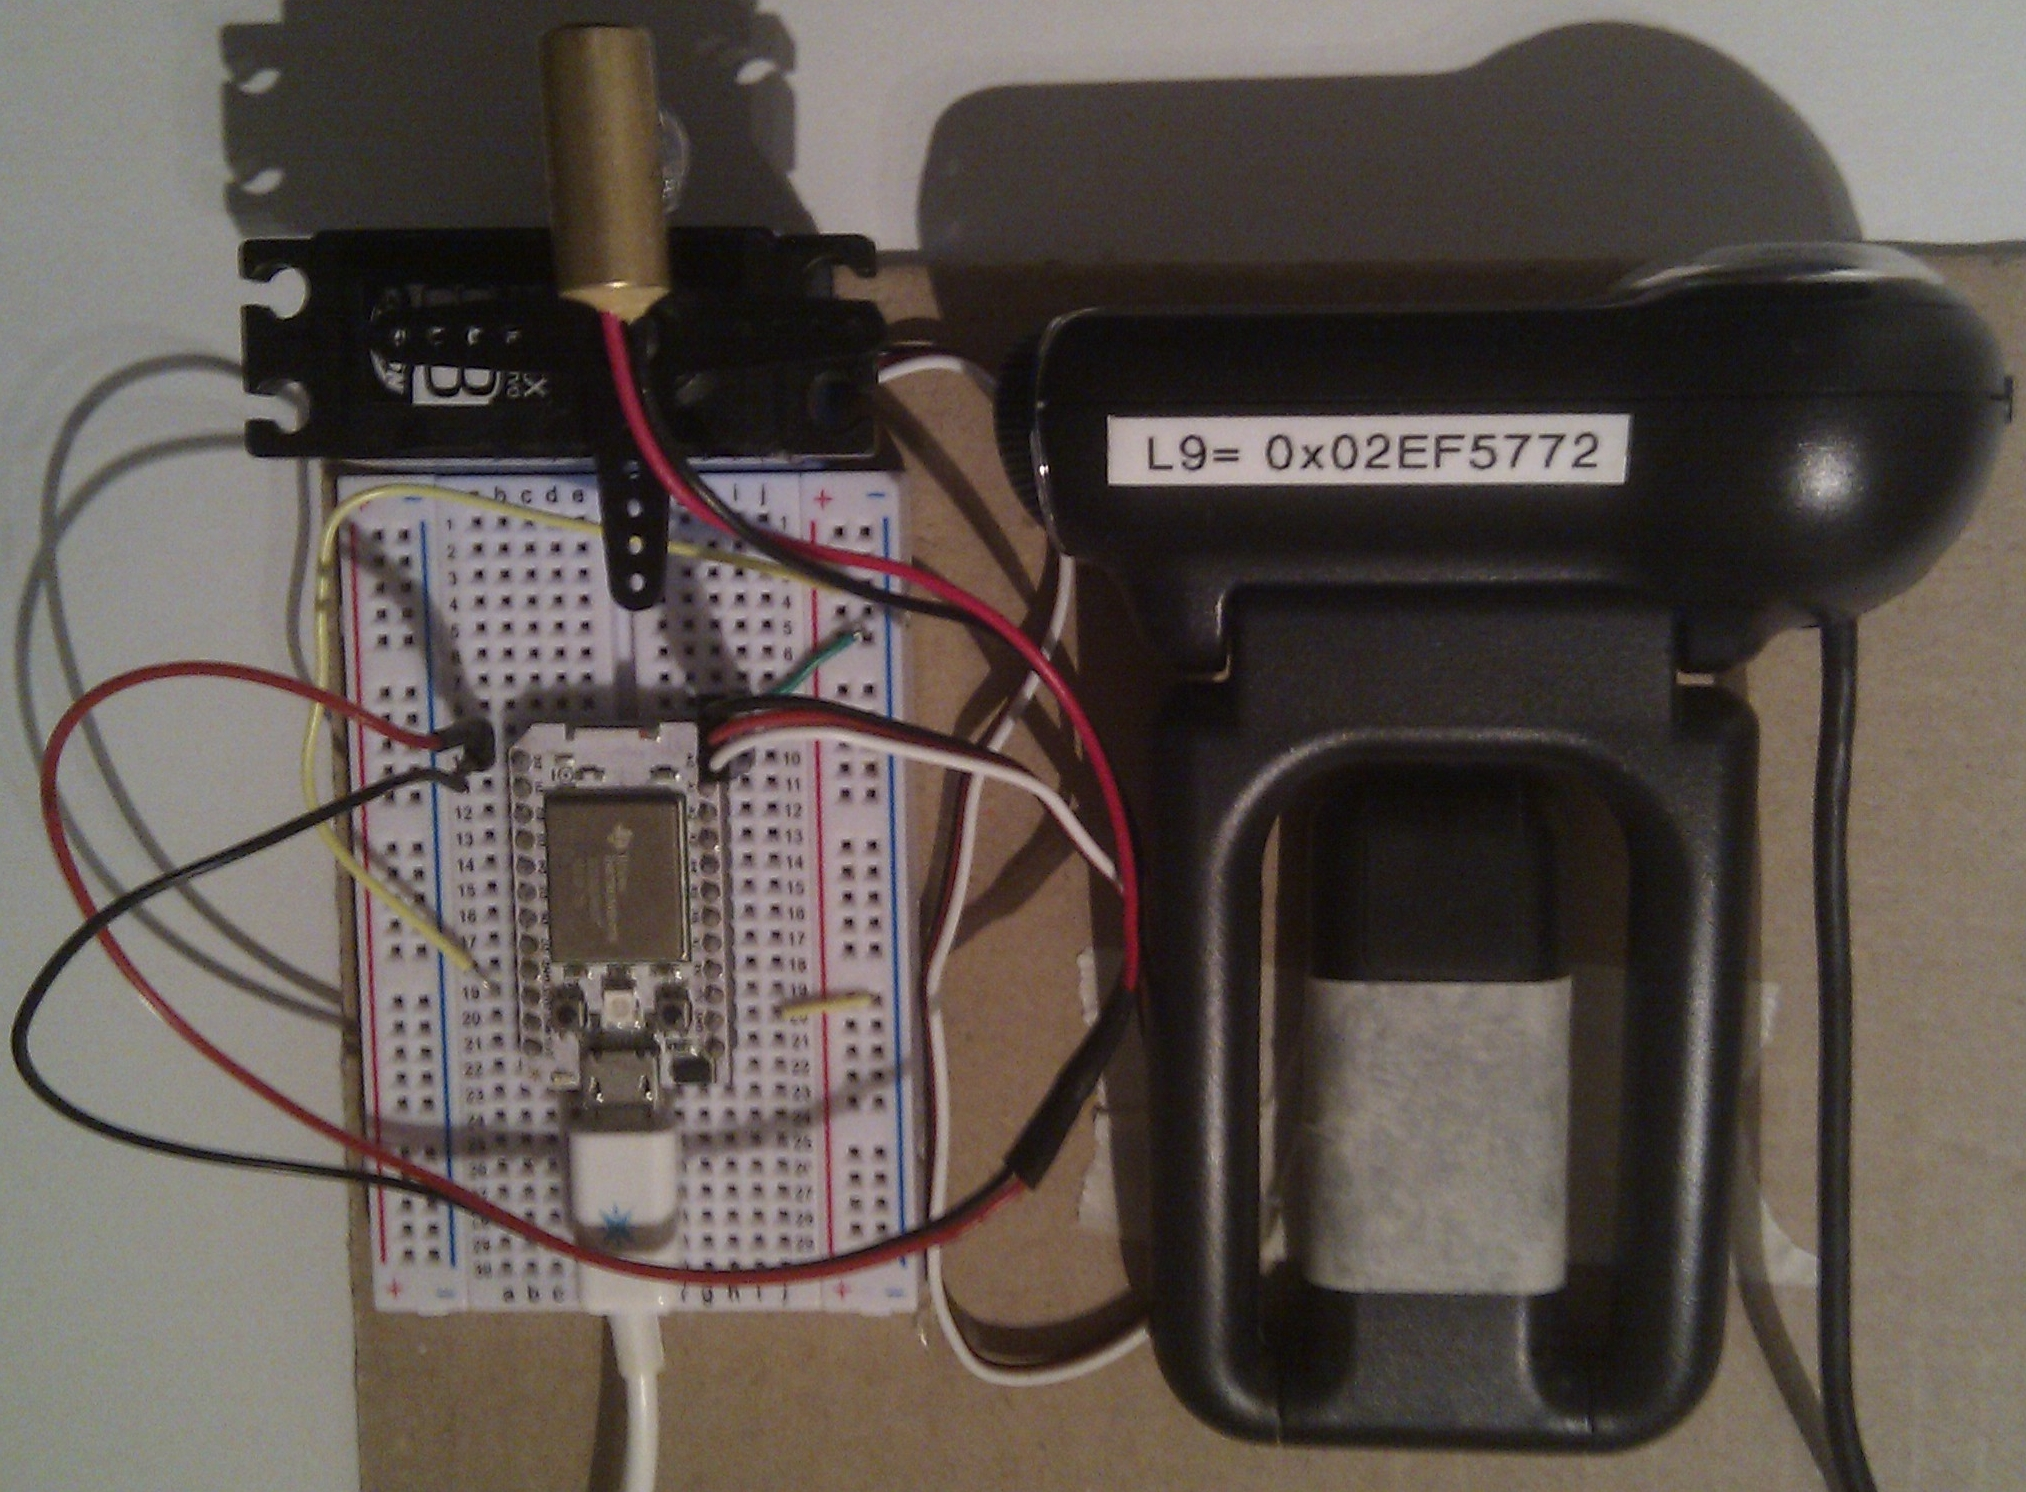
\includegraphics[height=4.5cm]{includes/hardware}
		\caption{reale Hardware}
	\end{subfigure}
	\caption{Aufbau der Hardware}
	\label{fig:hardware}
\end{figure}

\subsection{Softwarearchitektur}

Zur Implementierung der Software wurde die Programmiersprache \emph{C++} nach dem \emph{Standard von 2011} verwendet. Als Bibliotheken kamen \emph{OpenCV} und \emph{Qt} zum Einsatz. Eine Übersicht über alle Klassen ist in der Abbildung~\ref{fig:classes_all} zu finden. Im folgenden werden die einzelnen Komponenten der Software genauer betrachtet.

\begin{figure}[p]
	\centering
	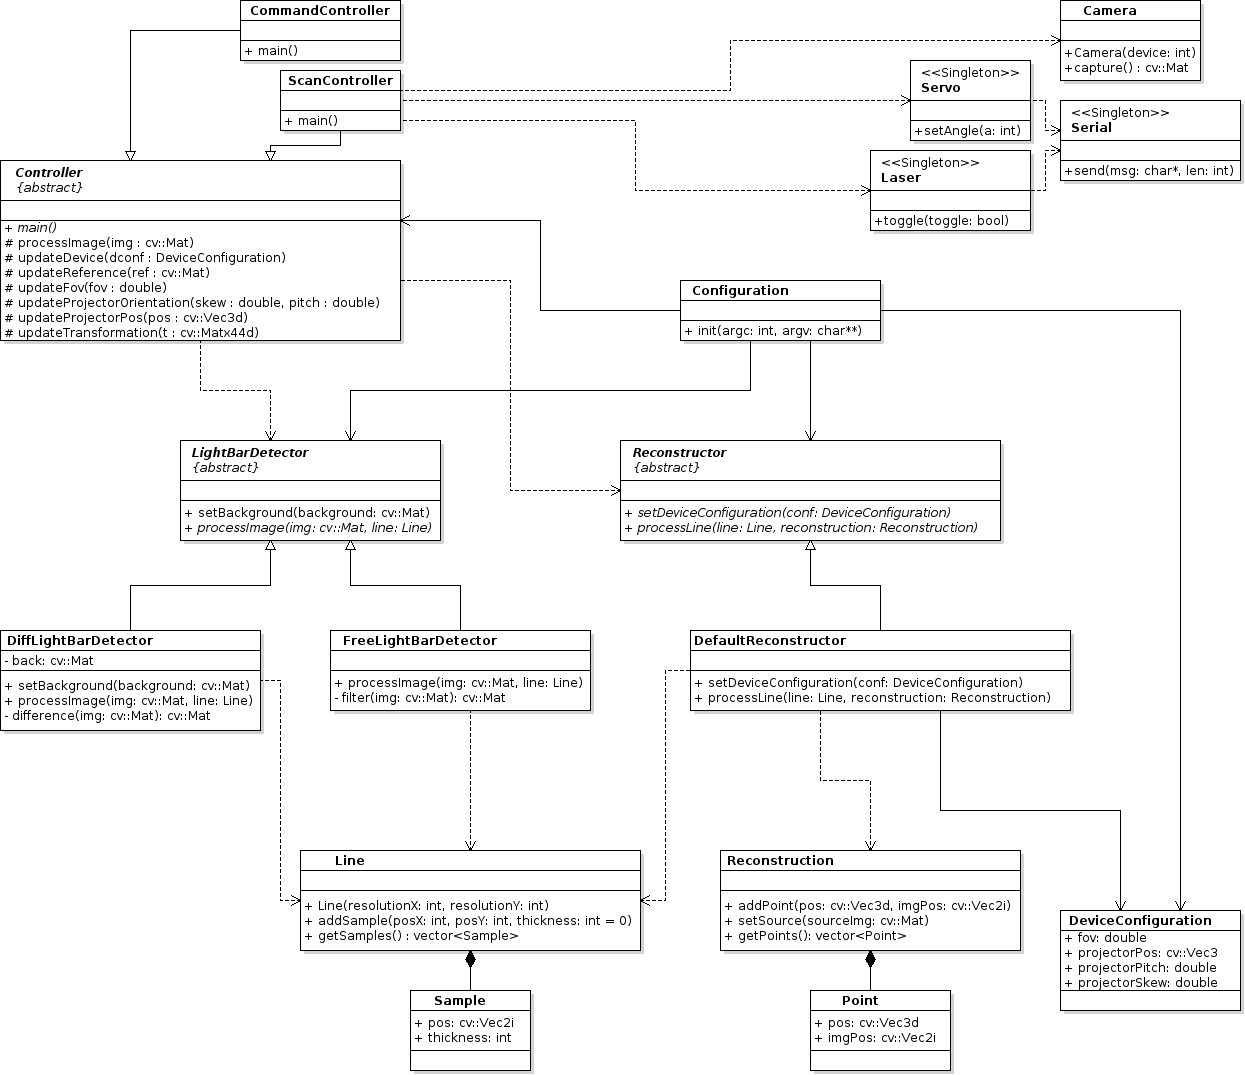
\includegraphics[width=\linewidth]{includes/classdiagram}
	\caption{Umfassendes Klassendiagramm}
	\label{fig:classes_all}
\end{figure}

\subsubsection{Grundlegende Datenstrukturen}

Zur Übertragung von Informationen zwischen den verschiedenen Komponenten werden die Datenstrukturen \texttt{Line}, \texttt{Reconstruction} und \texttt{DeviceConfiguration} verwendet. In Abbildung~\ref{fig:classes_base} sind die entsprechenden Klassen zu sehen. Die Funktion wird im folgenden etwas genauer beschrieben.

\begin{figure}
	\centering
	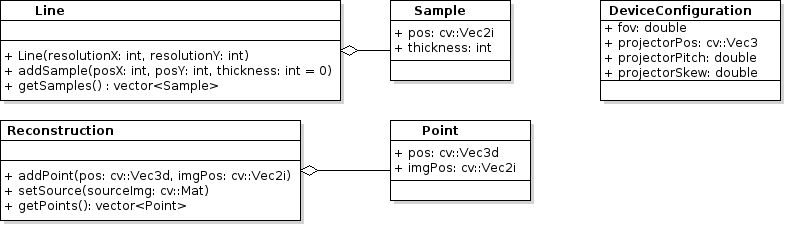
\includegraphics[width=\linewidth]{includes/classdiagram_base.png}
	\caption{Klassendiagramm zu den grundlegenden Datenstrukturen}
	\label{fig:classes_base}
\end{figure}

\vspace{0.5em}
\begin{tabular}{lp{10cm}}
	\texttt{DeviceConfiguration} &
		Die Struktur \texttt{DeviceConfiguration} speichert alle Werte zum Setup, die zur Rekonstruktion benötigt werden. Zusätzlich wird eine Transformationsmatrix mitgeführt, auf die später noch eingegangen wird.\\[1em]
	\texttt{Line}                &
		Die Datenstruktur \texttt{Line} entspricht einer Menge von Abtastungen der projizierten Linie. Sie Speichert dabei zusätzlich zu einer Liste von Abtastungen (Instanzen von \texttt{Sample}) die Auflösung des zugrunde liegenden Bildes.\\[1em]
	\texttt{Reconstruction}      &
		Die Klasse \texttt{Reconstruction} dient zum Speichern des endgültigen Ergebnisses der Rekonstruktion. Sie speichert somit eine Liste von rekonstruierten Punkten (Instanzen von \texttt{Point}). Zusätzlich hat die Klasse die Aufgabe, hinzugefügte rekonstruierte Punkte zur Ausgabe des Programms hinzuzufügen. Die entsprechenden Farben werden aus dem Referenzbild entnommen.
\end{tabular}

\subsubsection{Programmablauf}

\begin{figure}
	\centering
	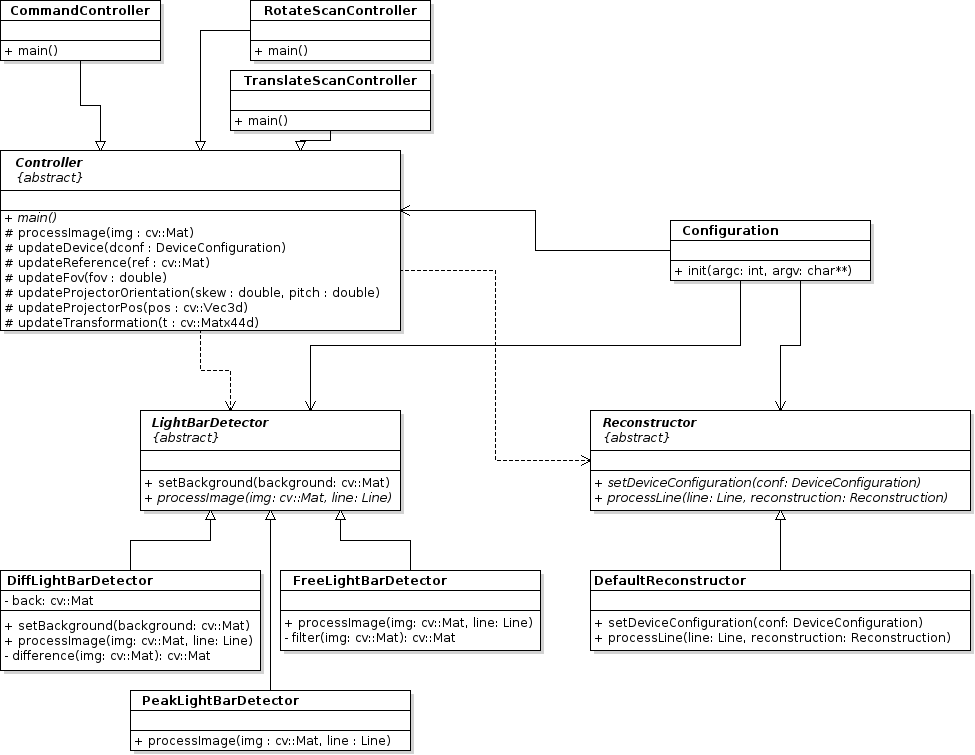
\includegraphics[width=\linewidth]{includes/classdiagram_control.png}
	\caption{Klassendiagramm zu den Steuereinheiten}
	\label{fig:classes_control}
\end{figure}

Nach Programmstart wird als erstes die Funktion \texttt{Configuration::init(int,char**)} aufgerufen. Diese analysiert die Argumente, die dem Programm übergeben wurden, und speichert das Ergebnis in den statischen Feldern der Klasse. Unter anderem wird dabei jeweils eine Instanz einer Spezialisierung von \texttt{Controller}, \texttt{LightBarDetector} und \texttt{Reconstructor} in den Feldern von \texttt{Configuration} abgelegt. Als nächstes wird die Methode \texttt{main()} der \emph{Steuerungsklasse}, also der Spezialisierung von \texttt{Controller}, aufgerufen, welche den Rest des Programmablaufes steuert.

\subsection{Steuerungsklassen}
\label{sec:controller}

\begin{figure}
	\centering
	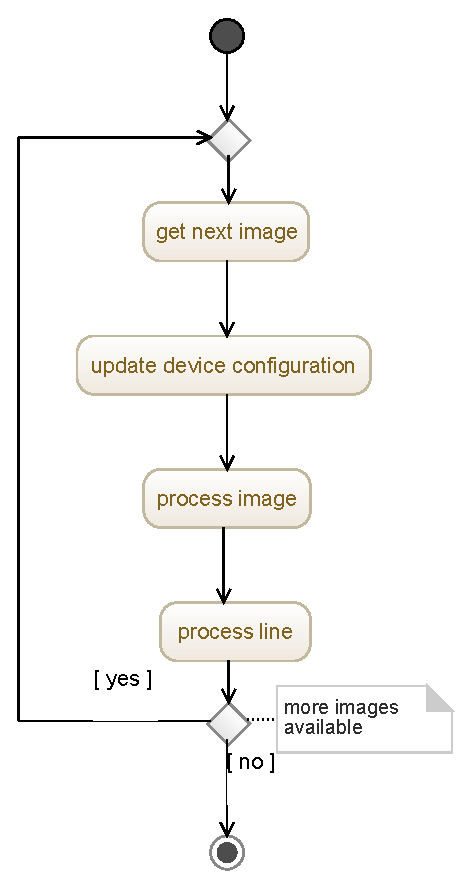
\includegraphics[width=0.4\linewidth]{includes/software_controller}
	\caption{Aktivitätsdiagramm zum Grundlegenden Programmablauf in den Steuerklassen.}
	\label{fig:software_controller}
\end{figure}

Der Ablauf, der von den verschiedenen Spezialisierungen von \texttt{Controller} vorgegeben wird, verfolgt dabei immer einen ähnlichen Ablauf, wie er auch in Abbildung~\ref{fig:software_controller} dargestellt wird. Der Controller durchläuft eine Schleife und beschafft sich in jedem Schleifendurchlauf die aktuelle Gerätekonfiguration (\texttt{DeviceConfiguration}), eine Aufnahme durch das entsprechende Setup und ggf. ein aktuelles Referenzbild. Danach übergibt es die Steuerung an die Linienerkennung (\texttt{LightBarDetector}) und dessen Ergebnis wird an den Rekonstruktionsalgorithmus (\texttt{Reconstructor}) übergeben.

Es existieren drei Spezialisierungen von \texttt{Controller}. Die einfachste Implementierung ist der \texttt{CommandController}, welcher Standardmäßig verwendet wird. Die Klasse liest die Standardeingabe oder die in den Argumenten definierte Datei Zeilenweise aus. Eine Zeile entspricht dabei einem Befehl, welcher ausgewertet und ausgeführt wird, bevor sich das Programm der nächsten Zeile zuwendet. In der Tabelle~\ref{tab:commands} können alle Befehle nachgelesen werden.

\begin{table}[p]
	\centering
	\begin{tabular}{lp{10cm}}
		\bfseries Befehl             & \bfseries Beschreibung\\
		\hline\hline
		\texttt{b <Datei>}           &
			Diese Zeile definiert die angegebene \emph{Datei} als neues Referenzbild.\\
		\hline
		\texttt{fov <Winkel>}        &
			Hier wird das \ac{FOV} auf den angegebenen \emph{Winkel} gesetzt. Der Winkel muss dabei in Radiant angegeben werden.\\
		\hline
		\texttt{pp <x> <y> <z>}      &
			Der Befehl setzt die Projektorposition $P$ auf den Punkt $(x,y,z)$.\\
		\hline
		\texttt{po <skew> <pitch>}   &
			Setzt die Werte $\theta$ und $\delta$ aus dem Modell. Die Winkel müssen dabei in Radiant angegeben werden.\\
		\hline
		\texttt{t <$m_1$> \dots <$m_{16}$>} &
			Setzt die Transformationsmatrix. Dabei wird die Matrix Zeilenweise aufgefüllt:
			\[ \begin{pmatrix}
				m_{1}  & m_{2}  & m_{3}  & m_{4}\\
				m_{5}  & m_{6}  & m_{7}  & m_{8}\\
				m_{9}  & m_{10} & m_{11} & m_{12}\\
				m_{13} & m_{14} & m_{15} & m_{16}
			\end{pmatrix} \]\\
		\hline
		\texttt{c <x> <fov> <pitch>} &
			Setzt die Projektorposition $P$ auf $(x,0,0)$, das \ac{FOV} auf den angegeben Winkel $\fov$, $\delta$ auf den angegeben Wert von \emph{pitch} und $\theta = 0$.\\
		\hline
		\texttt{<Datei>}             &
			Lässt die Rekonstruktion auf Basis der angegebenen Aufnahme laufen.\\
		\hline\hline
	\end{tabular}
	\caption{Unterstützte Befehle der Steuerungsklasse \texttt{CommandController}.}
	\label{tab:commands}
\end{table}

Die Klassen \texttt{RotateScanController} und \texttt{TranslateScanController} beschaffen die Aufnahmen hingehen direkt von der Hardware. Der \texttt{RotateScanController} rotiert dabei den Streifenprojektor um passende Aufnahmen zu erhalten. Der \texttt{TranslateScanController} macht eine Aufnahme und wartet anschließend auf eine Bestätigung des Benutzers, dass sich das zu scannende Objekt um eine vorher definierte Strecke bewegt hat, bevor er das nächste Bild aufnimmt.
Die Bewegung der Kamera bei Verwendung vom \texttt{TranslateScanController} wird dabei durch die Transformationsmatrix in der Gerätekonfiguration repräsentiert. Die rekonstruierten Punkte werden zum Abschluss als homogene Koordinaten mit dieser $4 \times 4$-Matrix multipliziert.

\subsection{Ansteuerung der Hardware}

\subsubsection{Ansteuerung des Mikrocontrollers}

Die Software steuert den Mikrocontroller über USB an, wobei sich dieser als virtuellen COM-Port ausgibt. Zur Kommunikation wird ein einfaches Protokoll verwendet, das zwei Byte lange Nachrichten an den Mikrocontroller sendet. Das erste Byte gibt den Befehl an, das zweite den Parameter. Die möglichen Befehle werden in der Tabelle~\ref{tab:protocol} aufgeführt.

\begin{table}
	\centering
	\begin{tabular}{|c|c|c|}
		\hline
		\bfseries 1. Byte & \bfseries 2. Byte & \bfseries Beschreibung \\
		\hline
		'm' & $\alpha \in [0,180]$ & Setzt die Servoposition auf $\alpha^\circ$\\
		\hline
		'l' & '0' oder '1' & Schaltet den Laser an ('1') bzw. aus ('0')\\
		\hline
	\end{tabular}
	\caption{Befehle zur Steuerung des Mikrocontrollers. Zeichen in einfachen Anführungszeichen stehen für den ASCII-Wert des Zeichens.}
	\label{tab:protocol}
\end{table}

Die Klasse \texttt{Serial} ermöglicht es Nachrichten an den Mikrocontroller zu senden. Die Klassen \texttt{Servo} und \texttt{Laser} implementieren die Steuerung von dem Servo bzw. Laser. Dabei werden Nachrichten in o.g. Form an den Mikrocontroller gesendet.

\subsubsection{Ansteuerung der Kamera}

Für das Auslesen von Bildern der Kamera ist die Klasse \texttt{Camera} zuständig, dabei liest ein extra Thread permanent Bilder von der Kamera.

Wenn ein anderer Thread die \texttt{capture}-Methode von \texttt{Camera} aufruft, blockiert er solange, bis der extra Thread das nächste Bild gelesen hat, und gibt dieses dann zurück. Das wird gemacht um sicherzustellen, dass immer das aktuellste Bild ausgelesen wird und nicht ein älteres Bild, das in einem Buffer der Kamera gespeichert wurde.


\subsection{Linienerkennung}

Die Linienerkennung arbeitet in zwei Schritten. Zuerst wird ein Binärbild erzeugt, wobei der Algorithmus entscheidet, welche Pixel zur Linie gehören und welche nicht. Im zweiten Schritt wird auf Basis des Binärbildes die Datenstruktur \texttt{Line} mit den vermeintlichen Abtastungen der Linie und, je nach Verfahren, auch mit der Breite der Linie gefüllt.

\subsubsection{Differenzbildung (Diff)}

\emph{Diff} benötigt zu jeder zu analysierenden Aufnahme ein Referenzbild; eine weitere Aufnahme der Szene, auf der die Linie nicht zu sehen ist. Das Referenzbild kann einmal zu Beginn aufgenommen werden, oder zwischen den einzelnen Aufnahmen der Linie. Durch die wiederholte Aufnahme des Referenzbildes wird das Verfahren toleranter gegenüber Beleuchtungsänderungen der Szene.
Als erstes wird die Differenz zwischen der Aufnahme und dem zugehörigen Referenzbild berechnet.
Liegt die Differenz für einen der Kanäle über einem bestimmten Schwellenwert (75), so wird davon ausgegangen, dass der Pixel zur Linie gehört.

Das Ergebnis ist ein Binärbild, mit dessen Hilfe im zweiten Schritt das \texttt{Line}-Objekt gefüllt wird. Dafür werden die Pixel das Binärbildes zeilenweise durchlaufen. Sobald ein Pixel gefunden wurde, der vermeintlich zur Linie gehört, wird dieser mit allen anschließenden markierten Pixel in der selben Zeile als ein Punkt auf Linie betrachtet. Die Position wird als Abtastung der Linie aufgenommen, wobei die Anzahl der hintereinander als Linie markierten Pixel als die Breite der Linie aufgefasst wird.

\subsubsection{Farbfilter (Free)}

Bei \emph{Free} wird zunächst für jeden Farbkanal der Durchschnitt über das gesamte Bild berechnet.
Auf Basis der Mittelwerte $m_{r/g/b}$ wird für jeden Farbkanal ein Schwellenwert $s_{r/g/b}$ bestimmt. Ist ein Kanal eines Pixels kleiner als der entsprechende Schwellenwert, dann gehört der Pixel nicht zur Linie.
Unter der Annahme, dass die Werte der Farbkanäle in dem Intervall $[0,255]$ liegen, wird der Schwellenwert dabei wie folgt berechnet:
\begin{align*}
	s_r &= m_r + \frac{255 - m_r}{2}\\
	s_i &= m_i - \frac{255 - m_i}{2}, i \in \{g,b\}
\end{align*}

Der zweite Schritt des Verfahrens verläuft Analog zu Diff.

\subsubsection{Erweiterter Farbfilter (Peak)}

\emph{Peak} ist das experimentellste der Verfahren und wurde noch nicht genügend getestet und optimiert. Es basiert auf dem Verfahren Free.
Anstatt einen Mittelwerte über dem gesamten Bild zu berechnen, wird ein Mittelwert in einer kleinen rechteckigen Umgebung jedes Pixels bestimmt. Aus diesem Mittelwert $m$ und der Farbe des Pixels $c$ wird eine Wahrscheinlichkeit $p \in [0, 1]$ des Punktes berechnet mit der der Pixel zur Linie gehört. Wenn $p$ größer ist, als ein festgelegter Grenzwert, wird davon ausgegangen, dass der Punkt zur Linie gehört.
Zur Berechnung von $p$ werden dabei zunächst die Zwischenergebnisse $r_{r/g/b}$ berechnet, um diese gewichtet in $p$ einzubringen:
\begin{align*}
	r_i &= \begin{cases}
	0.5                         &\text{, falls } m_i = 255\\
	\frac{c_i - m_i}{255 - m_i} &\text{, sonst}
	\end{cases}, i \in \{r,g,b\}\\
	p &= \max(0,6 \cdot r_r + 0,2 \cdot r_g + 0,2 \cdot r_b, 0)
\end{align*}

Im zweiten wird auf dem gefilterten Bild ein \emph{Gaußfilter} angewendet, um danach nur Pixel als Bestandteil der Linie zu markieren, die ein lokales Maximum in einer Dimension annehmen. Diese Änderung soll es ermöglichen, auch mit horizontalen oder anders rotierten Linien zu arbeiten.

Ergänzend wenden wir bei dieser Methode einen weiteren Schritt an. Dabei werden alle Markierungen entfernt, bei denen der Pixel keine markierten Nachbarpixel besitzt, da Pixel auf der Linie in der Regel auch Nachbarpixel haben sollten, die ebenfalls auf der Linie liegen.

\subsection{Rekonstruktion}

Nachdem die Laserlinie erkannt wurde, werden die vermeintlichen Pixel der erkannten Linie in Objektpunkte überführt. Dies geschieht durch die Klasse \texttt{DefaultReconstructor}, welche derzeit die einzige Spezialisierung von \texttt{Reconstructor} darstellt.

Dazu werden die Formeln aus Abschnitt~\ref{sec:basics} angewendet, um für jeden Pixel zunächst die normalisierten Bildkoordinaten, die Entfernung $h$ und danach den Objektpunkt $X$ zu bestimmen. Daraufhin werden die erhalten Punkte mithilfe der Transformationsmatrix transformiert und an die Klasse \texttt{Reconstruction} weiter gegeben, welche sie letztendlich ausgibt.
	
%\begin{table}[p]
%	\centering
%	\begin{tabular}{lp{10cm}}
%		\bfseries Klasse                & \bfseries Funktion\\
%		\hline\hline
%		\texttt{CommandController}      &
%			Diese Klasse stellt als Spezialisierung von \texttt{Controller} eine Steuerungsklasse da, welche eingehende Befehle verarbeitet. Eine Liste der Befehl ist in \Fref{tab:commands} zu finden.\\
%		\hline
%		\texttt{Configuration}          &
%			Diese Klasse ist eine rein statische Klasse. Sie analysiert nach Programmstart die Argumente, die an das Programm übergeben wurden, und speichert die Einstellungen für die weitere Programmausführung.\\
%		\hline
%		\texttt{Controller}             &
%			Diese abstrakte Klasse bildet die Basis für alle Steuerungsklassen und definiert Funktionen mit denen die Steuerungsklasse ihre Arbeit verrichten kann. Eine Steuerungsklasse bestimmt den Programmablauf und ist dabei für die Beschaffung der Setup-Informationen und Bilder verantwortlich.\\
%		\hline
%		\texttt{DefaultReconstructor}   &
%			Als Spezialisierung von \texttt{Reconstructor} stellt diese Klasse den einzigen Rekonstruktionsalgorithmus da.\\
%		\hline
%		\texttt{DeviceConfiguration}    &
%			Diese Struktur speichert alle Werte zum Setup, die zur Rekonstruktion benötigt werden. Dazu gehört beispielsweise die Position und Ausrichtung des Projektors. Zusätzlich wird eine Transformationsmatrix mitgeführt, auf dessen Basis Punkte nach der Triangulation transformiert werden.\\
%		\hline
%		\texttt{DiffLightBarDetector}   &
%			Als Spezialisierung von \texttt{LightBarDetector} stellt diese Klasse eine Linienerkennung da.  Nähere Informationen in \Fref{sec:line_diff}.\\
%		\hline
%		\texttt{FreeLightBarDetector}   &
%			Als Spezialisierung von \texttt{LightBarDetector} stellt diese Klasse eine Linienerkennung da. Nähere Informationen in \Fref{sec:line_free}.\\
%		\hline
%		\texttt{LightBarDetector}       &
%			Diese abstrakte Klasse dient als Basis für alle Implementierungen zur Detektion der Laserlinie.\\
%		\hline
%		\texttt{Line}                   &
%			Diese Datenstruktur entspricht einer Menge von Abtastungen der projizierten Linie. Sie Speichert dabei eine Liste von Indizes, dessen Pixel zur Laserlinie gehören, und die Auflösung des zugrunde liegenden Bildes. Die Indizes werden dabei in Instanzen von \texttt{Sample} abgelegt.\\
%		\hline
%		\texttt{Reconstruction}         &
%			Diese Klasse speichert das endgültige Ergebnis der Rekonstruktion. Außerdem kümmert sie sich um die Ausgabe der rekonstruierten Punkte.\\
%		\hline
%		\texttt{Reconstructor}          &
%			Diese abstrakte Klasse dient als Basis für alle Implementierungen zur Rekonstruktion der Objektpunkte auf Basis der bereits erkannten Laserlinie.\\
%		\hline
%		\texttt{RotateScanController}   &
%			Diese Klasse stellt als Spezialisierung von \texttt{Controller} eine Steuerungsklasse da. Sie kann verwendet werden, um Objekte mit Hilfe einer Drehung des Projektors zu scannen.\\
%		\hline
%		\texttt{TranslateScanController} &
%			Diese Klasse stellt als Spezialisierung von \texttt{Controller} eine Steuerungsklasse da. Sie kann verwendet werden, um Objekte mit Hilfe einer schrittweisen Bewegung an der Kamera vorbei zu scannen.\\
%		\hline\hline
%	\end{tabular}
%	\caption{Umfassende Tabelle der Klassen}
%	\label{tab:classes_all}
%\end{table}

% ---------------------------------------------------------------------------- %

\section{Auswertung}
\label{sec:evaluation}

Im Folgenden werden verschiedene Seiten eines ''Rubik's Cube'' auf verschiedene Entfernungen gescannt. Es wurden die rote, grüne, blaue, gelbe und orange Seite in 300~mm Entfernung, sowie die blaue Seite in 200~mm, 400~mm und 500~mm Entfernung vermessen. Die Zugehörigkeit eines Messpunktes wird anhand seiner Farbe, die aus dem Referenzbild entnommen wurde, bestimmt. Da die Scans vor weißem Hintergrund durchgeführt wurden, wurde die weiße Seite des ''Rubik's Cube'' nicht gescannt.

\begin{figure}[H]
	\centering
	\begin{subfigure}{0.45\textwidth}
		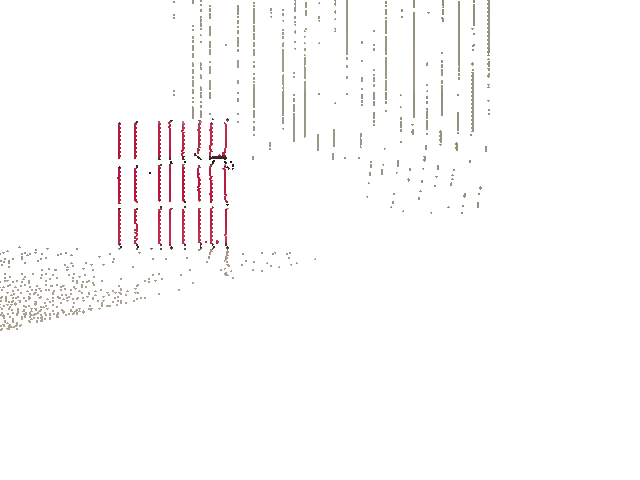
\includegraphics[width=\textwidth,frame]{includes/diff_red_cam.png}
		\caption{komplette Punktwolke aus Sicht der Kamera}
	\end{subfigure}
	\hfill
	\begin{subfigure}{0.45\textwidth}
		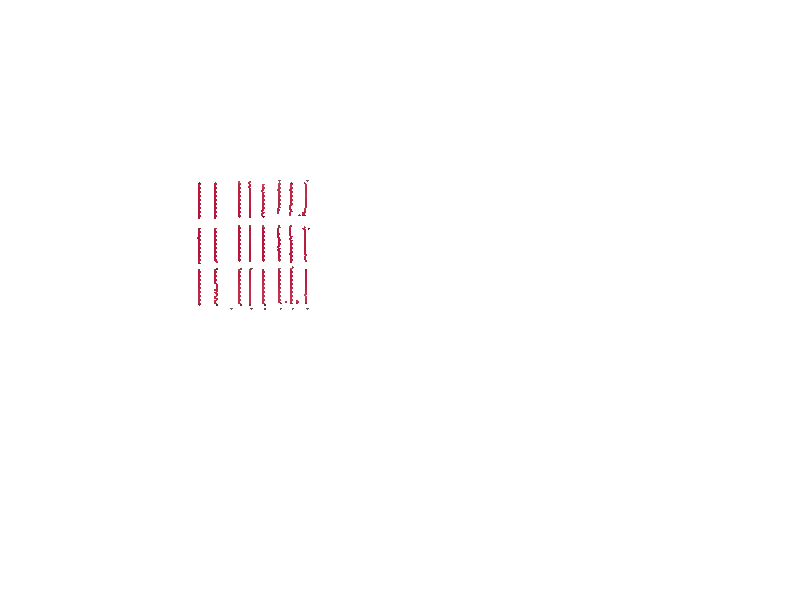
\includegraphics[width=\textwidth,frame]{includes/diff_only_red_cam.png}
		\caption{Punktwolke der Punkte, die zum Würfel gehören, aus Sicht der Kamera}
	\end{subfigure}
	\begin{subfigure}{0.45\textwidth}
		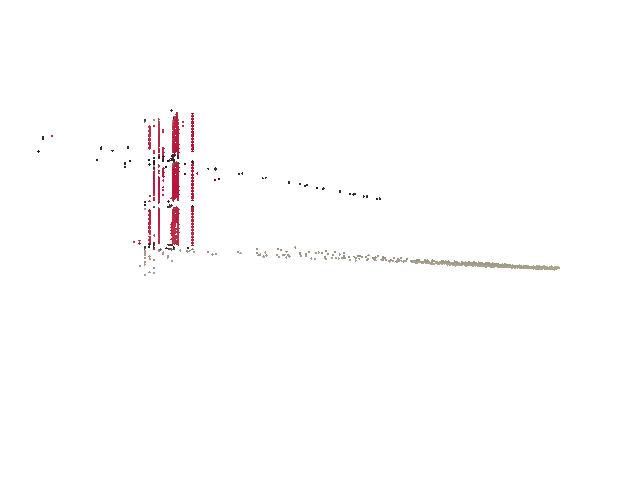
\includegraphics[width=\textwidth,frame]{includes/diff_red_pos1.png}
		\caption{komplette Punktwolke von der Seite \\ \mbox{}}
	\end{subfigure}
	\hfill
	\begin{subfigure}{0.45\textwidth}
		
\includegraphics[width=\textwidth,frame]{includes/diff_only_red_pos1.png}
		\caption{Punktwolke der Punkte, die zum Würfel gehören, von der Seite}
	\end{subfigure}
	\caption{Punktwolken eines Scans mit Diff-Linienerkennung der roten Seite des ''Rubik's Cube'' in 300~mm Entfernung}
\end{figure}

\begin{figure}[H]
	\centering
	\begin{subfigure}{0.45\textwidth}
		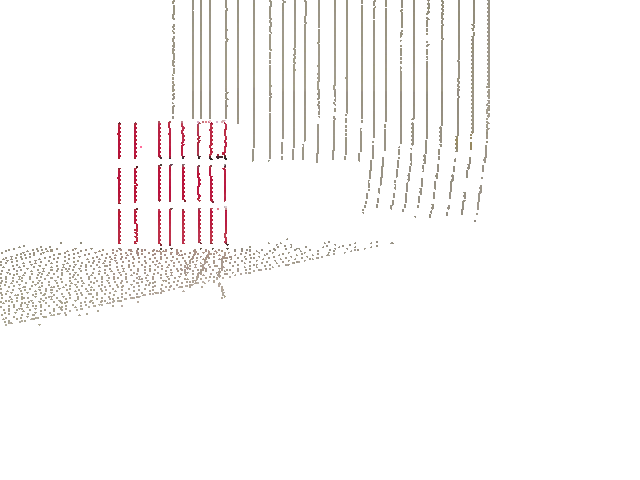
\includegraphics[width=\textwidth,frame]{includes/free_red_cam.png}
		\caption{komplette Punktwolke aus Sicht der Kamera}
	\end{subfigure}
	\hfill
	\begin{subfigure}{0.45\textwidth}
		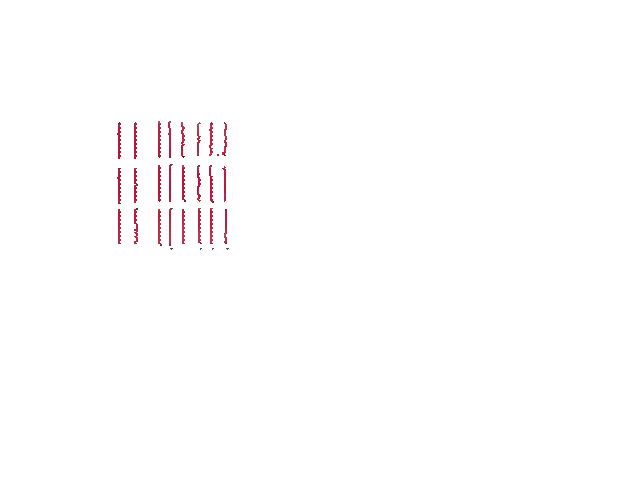
\includegraphics[width=\textwidth,frame]{includes/free_only_red_cam.png}
		\caption{Punktwolke der Punkte, die zum Würfel gehören, aus Sicht der Kamera}
	\end{subfigure}
	\begin{subfigure}{0.45\textwidth}
		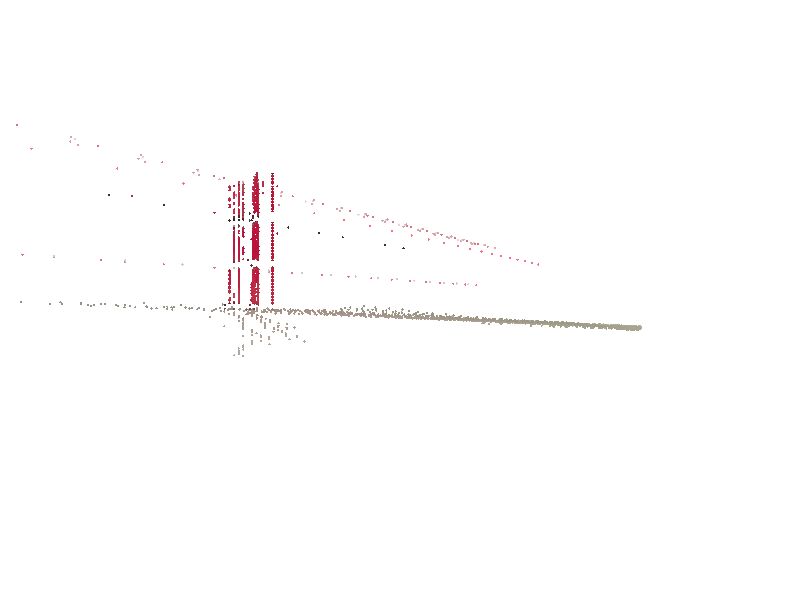
\includegraphics[width=\textwidth,frame]{includes/free_red_pos1.png}
		\caption{komplette Punktwolke von der Seite \\ \mbox{}}
	\end{subfigure}
	\hfill
	\begin{subfigure}{0.45\textwidth}
		
\includegraphics[width=\textwidth,frame]{includes/free_only_red_pos1.png}
		\caption{Punktwolke der Punkte, die zum Würfel gehören, von der Seite}
	\end{subfigure}
	\caption{Punktwolken eines Scans mit Free-Linienerkennung der roten Seite des ''Rubik's Cube'' in 300~mm Entfernung}
\end{figure}

\begin{figure}[H]
	\centering
	\begin{subfigure}{0.45\textwidth}
		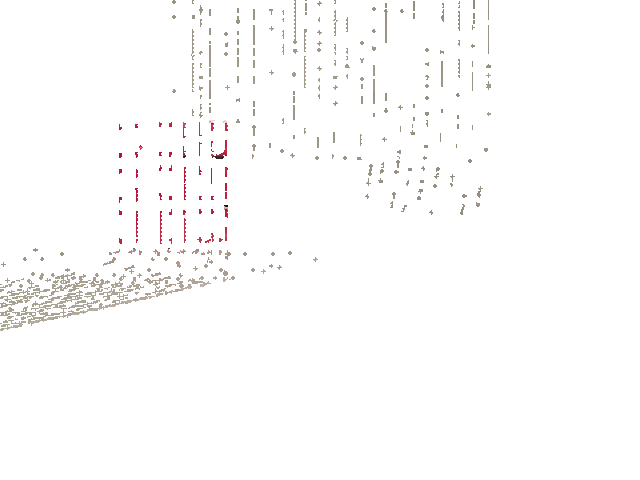
\includegraphics[width=\textwidth,frame]{includes/peak_red_cam.png}
		\caption{komplette Punktwolke aus Sicht der Kamera}
	\end{subfigure}
	\hfill
	\begin{subfigure}{0.45\textwidth}
		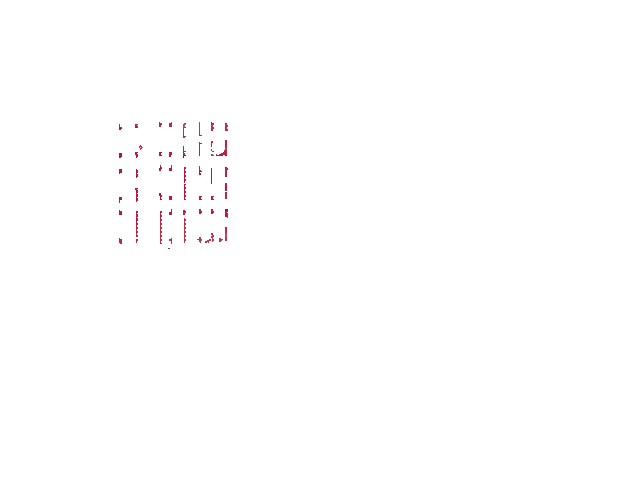
\includegraphics[width=\textwidth,frame]{includes/peak_only_red_cam.png}
		\caption{Punktwolke der Punkte, die zum Würfel gehören, aus Sicht der Kamera}
	\end{subfigure}
	\begin{subfigure}{0.45\textwidth}
		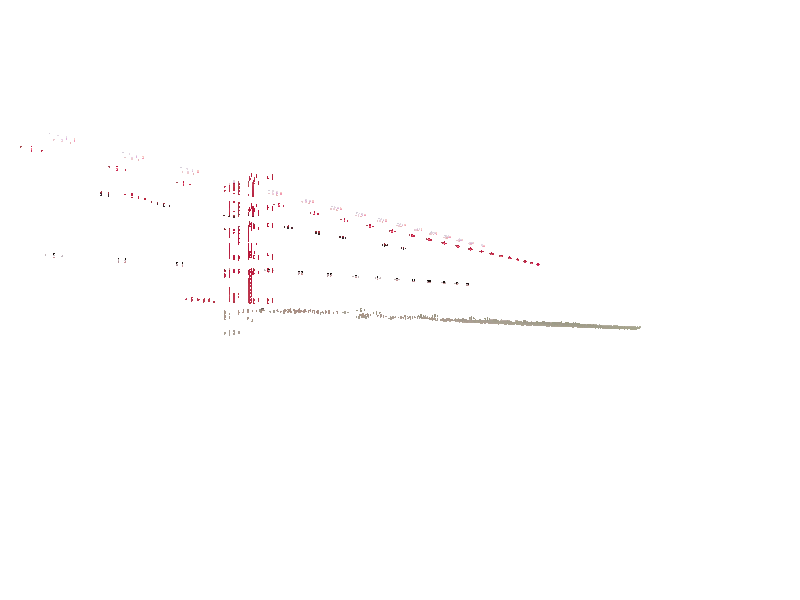
\includegraphics[width=\textwidth,frame]{includes/peak_red_pos1.png}
		\caption{komplette Punktwolke von der Seite \\ \mbox{}}
	\end{subfigure}
	\hfill
	\begin{subfigure}{0.45\textwidth}
		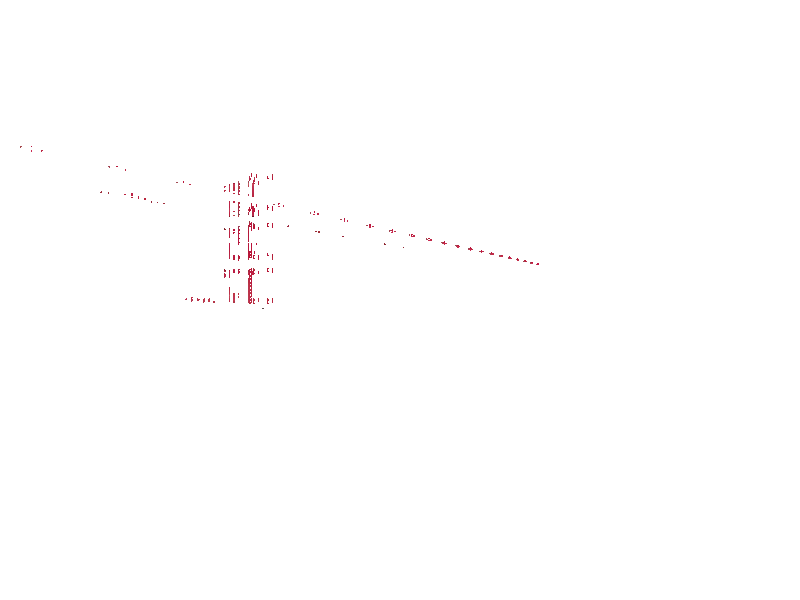
\includegraphics[width=\textwidth,frame]{includes/peak_only_red_pos1.png}
		\caption{Punktwolke der Punkte, die zum Würfel gehören, von der Seite}
	\end{subfigure}
	\caption{Punktwolken eines Scans mit Peak-Linienerkennung der roten Seite des ''Rubik's Cube'' in 300~mm Entfernung}
\end{figure}


\subsection{Wiederholte Messungen}
\label{sec:reps}

Zunächst wurde die blaue Seite des ''Rubik's Cube'' zehn mal in 300~mm Entfernung vermessen, um die Abweichungen zwischen zwei Messungen zu bestimmen. In Tabelle \ref{tab:reps} sind die Ergebnisse aufgeführt. In der Spalte ''Anzahl'' steht jeweils die Anzahl der Punkte, die zum Würfel gehören. Unter ''Avg'' ist das $20 \%$ gestutzte Mittel und unter ''Stdabw'' die Standardabweichung aller gemessenen Entfernungen aufgeführt.

Es fällt auf, dass sich die Werte zwischen verschiedenen Messungen kaum unterscheiden, aber es zwischen den Linienerkennungen z.T. große Unterschiede gibt. So findet Diff die meisten Punkte auf dem Würfel und Peak hat mit Abstand die höchste Standardabweichung ( fast 100 mal höher als bei Free)

Wie man in Abbildung \ref{fig:cols} sehen kann, spiegelt sich der Laser in dem Cube. Die Diff-Linienerkennung erkennt, im Gegensatz zur Free-Linienerkennung, die Spiegelung als Linie. Das erklärt sowohl warum Diff mehr Punkte erkennt, als auch warum diese eine höhere Streuung aufweisen.
Peak erkennt viele falsche Punkte an der Kante des Würfels, was zu einer hohen Streuung führt.

Zusätzlich fällt auf, dass die durchschnittliche Entfernung von allen drei Linienerkennungen 38mm - 42mm ($12,5\%-14\%$) größer ist als erwartet (300~mm), siehe dazu Abschnitt \ref{sec:dists}.

\begin{table}[H]
	\centering
	Diff-Linienerkennung \\
	\begin{tabular}{c|c|c|c}
		Wiederholung & Anzahl & Avg (mm) & Stdabw (mm) \\ \hline
		1 & 825 & 338.851 & 15.1979 \\
		2 & 829 & 338.511 & 14.199 \\
		3 & 807 & 338.858 & 13.7228 \\
		4 & 818 & 338.825 & 15.9249 \\
		5 & 851 & 338.931 & 15.6883 \\
		6 & 857 & 338.927 & 13.3769 \\
		7 & 832 & 338.541 & 14.5219 \\
		8 & 847 & 338.688 & 14.5952 \\
		9 & 825 & 338.494 & 13.6795 \\
		10 & 830 & 338.469 & 16.8786 \\
	\end{tabular} \\
	\vspace{1em}
	Free-Linienerkennung \\
	\begin{tabular}{c|c|c|c}
		Wiederholung & Anzahl & Avg (mm) & Stdabw (mm) \\ \hline
		1 & 363 & 340.952 & 2.76884 \\
		2 & 365 & 340.923 & 2.97673 \\
		3 & 344 & 341.142 & 2.75016 \\
		4 & 336 & 341.02 & 2.68906 \\
		5 & 365 & 340.75 & 2.59545 \\
		6 & 350 & 340.738 & 2.71992 \\
		7 & 354 & 340.867 & 2.93117 \\
		8 & 353 & 340.764 & 2.9996 \\
		9 & 351 & 340.737 & 2.80947 \\
		10 & 354 & 341.064 & 2.97436 \\
	\end{tabular} \\
	\vspace{1em}
	Peak-Linienerkennung \\
		\begin{tabular}{c|c|c|c}
		Wiederholung & Anzahl & Avg (mm) & Stdabw (mm) \\ \hline
		1 & 647 & 341.039 & 238.143 \\
		2 & 618 & 341.134 & 225.873 \\
		3 & 614 & 341.748 & 216.396 \\
		4 & 662 & 341.748 & 232.574 \\
		5 & 698 & 341.264 & 235.846 \\
		6 & 638 & 339.998 & 241.649 \\
		7 & 681 & 340.775 & 241.377 \\
		8 & 651 & 340.45 & 249.112 \\
		9 & 700 & 341.317 & 221.319 \\
		10 & 634 & 341.085 & 241.876 \\
		\end{tabular} \
	\caption{Scans der blauen Seite in 300~mm Entfernung}
	\label{tab:reps}
\end{table}

\subsection{Verschiedene Farben}
\label{sec:cols}

Als nächstes wurden die verschiedenen Seiten des ''Rubik's Cube'' gescannt, um die Farbabhängigkeit der Linienerkennungen zu überprüfen. Die Ergebnisse sind in Tabelle \ref{tab:colors} zu finden. Sie ist analog zur Tabelle \ref{tab:reps} aus Abschnitt \ref{sec:reps} aufgebaut, mit dem Unterschied, dass pro Zeile nicht die Punkte aus einer Messung, sondern aus zehn Messungen betrachtet werden.

Es fällt auf, dass bei der roten Seite alle Linienerkennungen gute Ergebnisse liefern (niedrige Streuung der Messpunkte) und auch die Anzahl der gefunden Punkte und die Durchschnittsentfernung nahe beieinanderliegen. Zusätzlich liefern die Linienerkennungen bei Gelb vergleichsweise schlechte Ergebnisse (hohe Streuung). Bei den anderen Farben unterscheiden sich die Linienerkennungen z.T. stark, so liefert Diff bei grün die schlechtesten Ergebnisse, wohingegen Free mit orange starke Probleme hat und Peak hat bei blau die höchste Standardabweichung. Bei Free und der orangen Seite ist nicht nur die Standardabweichung extrem hoch, sondern auch die Anzahl der gefundenen Punkte ist ungefähr acht mal größer als bei grün oder blau, das heißt, dass ca. $\frac{7}{8}$ der erkannten Punkte nicht zur Linie gehören. Das liegt daran, dass Free den Mittelwert über das gesamte Bild bildet und anhand der Abweichung eines Punktes zum Mittelwert bestimmt, ob ein Punkt zur Linie gehört oder nicht. Die orange Seite verändert den Mittelwert so, dass auch Punkte, die nicht zur Linie gehören erkannt werden, siehe Abbildung \ref{fig:cols}. Ähnlich verhält es sich bei Peak, da werden falsche Punkte hauptsächlich am Rand des ''Rubik's Cube'' erkannt.

Insgesamt scheint Diff farbunabhängiger zu sein, da die Durchschnittsentfernung ziemlich konstant ist und auch die Anzahl der gefundenen Punkte weniger stark schwankt, als bei Free oder Peak. 


\begin{table}[H]
	\centering
	Diff-Linienerkennung \\
	\begin{tabular}{c|c|c|c}
		Farbe & Anzahl & Avg (mm) & Stdabw (mm) \\ \hline
		Rot & 6565 & 338.14 & 3.6842 \\
		Grün & 8806 & 337.897 & 88.2139 \\
		Blau & 8321 & 338.722 & 14.8228 \\
		Gelb & 7085 & 338.112 & 39.4331 \\
		Orange & 6336 & 338.249 & 7.50314 \\
	\end{tabular} \\
	\vspace{1em}
	Free-Linienerkennung \\
		\begin{tabular}{c|c|c|c}
		Farbe & Anzahl & Avg (mm) & Stdabw (mm) \\ \hline
		Rot & 6439 & 338.035 & 3.4453 \\
		Grün & 3534 & 340.808 & 6.28125 \\
		Blau & 3535 & 340.892 & 2.82819 \\
		Gelb & 10824 & 338.69 & 77.4283 \\
		Orange & 29063 & 347.896 & 205.929 \\
	\end{tabular} \\
	\vspace{1em}
	Peak-Linienerkennung \\
		\begin{tabular}{c|c|c|c}
		Farbe & Anzahl & Avg (mm) & Stdabw (mm) \\ \hline
		Rot & 5795 & 339.622 & 55.6553 \\
		Grün & 4437 & 341.713 & 152.687 \\
		Blau & 6543 & 341.249 & 234.736 \\
		Gelb & 5838 & 340.121 & 106.932 \\
		Orange & 4317 & 340.104 & 85.2112 \\
	\end{tabular} \
	\caption{Scans der verschiedener Seiten in 300~mm Entfernung}
	\label{tab:colors}
\end{table}


\begin{figure}[H]
	\centering
	\begin{tabular}{l|l|l|l}
		Bild der Kamera & erkannte Linie nach & erkannte Linie nach  & erkannte Linie nach \\
		& Diff-Linienerkennung & Free-Linienerkennung & Peak-Linienerkennung \\
		\hline 
		& & \\
		\raisebox{0.75em}{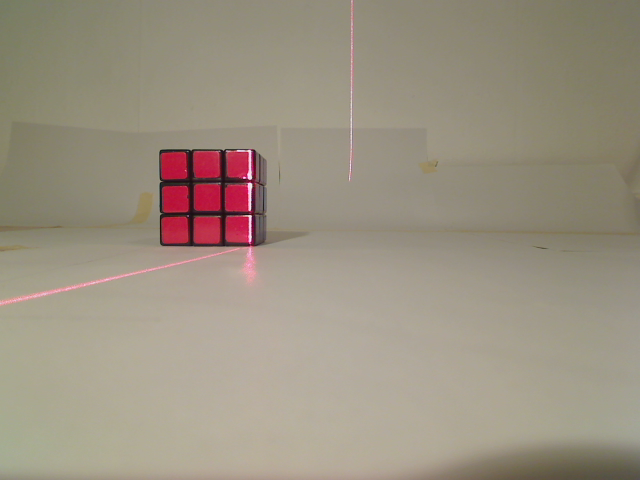
\includegraphics[height=6em]{includes/red_0.png}} & 
		\raisebox{0.75em}{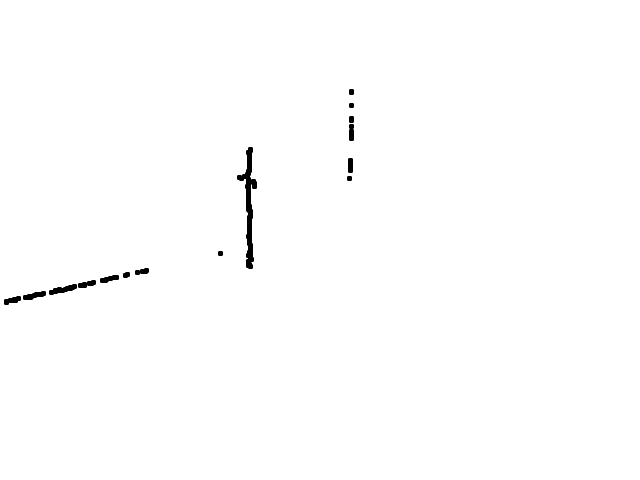
\includegraphics[height=6em]{includes/red_0_diff.png}} &
		\raisebox{0.75em}{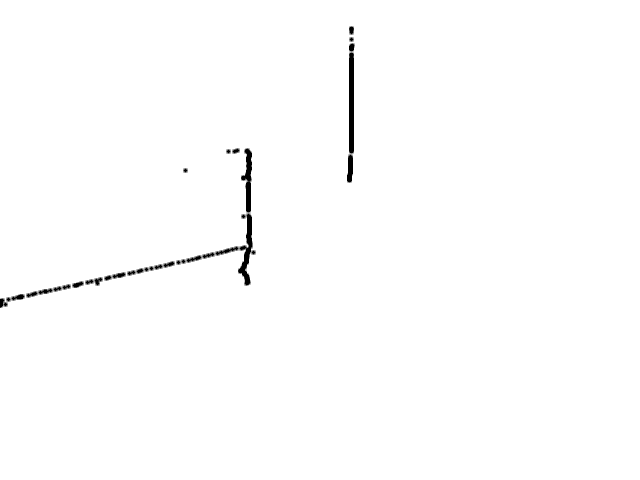
\includegraphics[height=6em]{includes/red_0_free.png}} &
		\raisebox{0.75em}{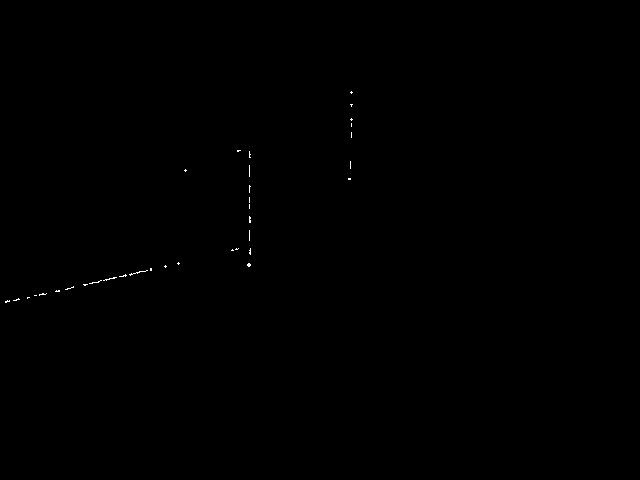
\includegraphics[height=6em]{includes/red_0_peak.png}} \\
		\hline
		& & \\
		\raisebox{0.75em}{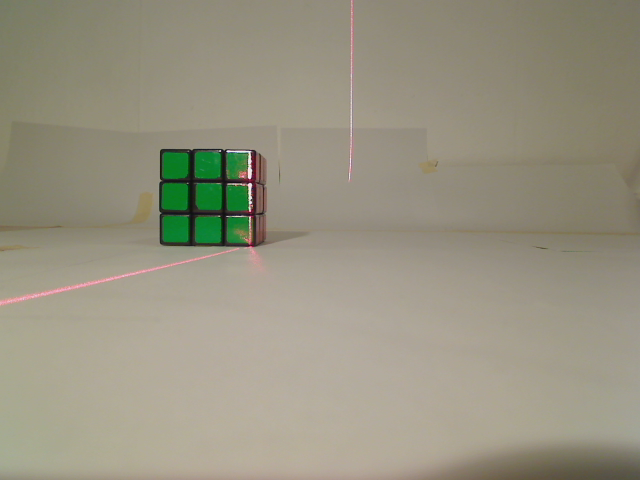
\includegraphics[width=.22\textwidth]{includes/green_0.png}} &
		\raisebox{0.75em}{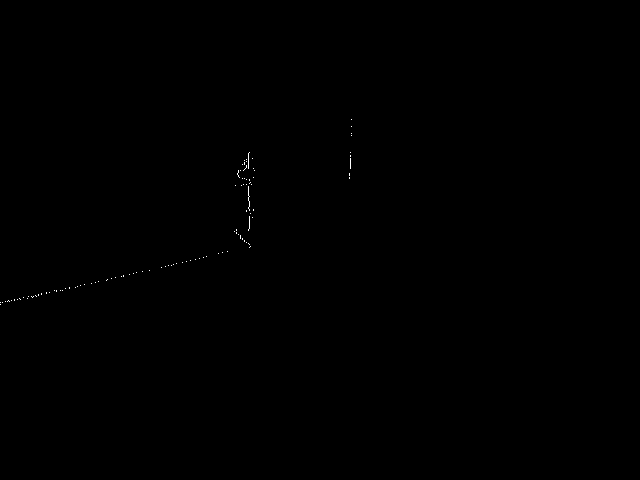
\includegraphics[width=.22\textwidth]{includes/green_0_diff.png}} &
		\raisebox{0.75em}{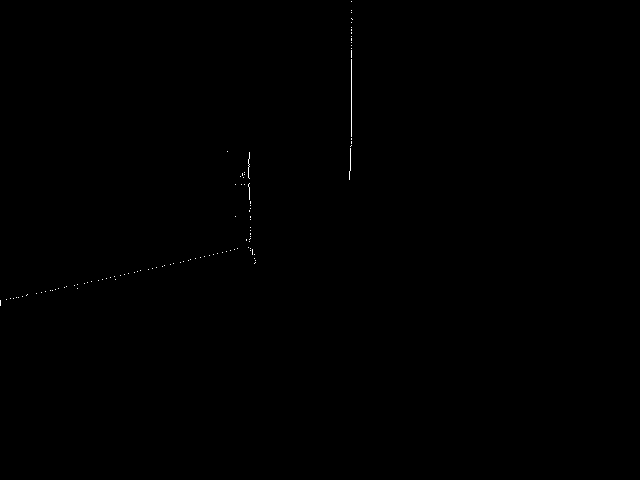
\includegraphics[width=.22\textwidth]{includes/green_0_free.png}} &
		\raisebox{0.75em}{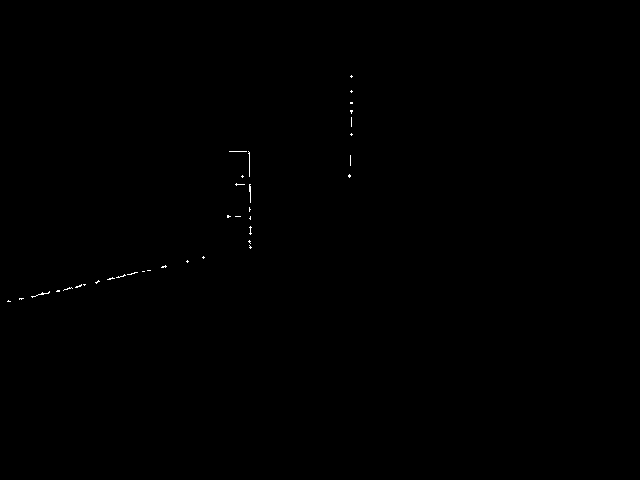
\includegraphics[width=.22\textwidth]{includes/green_0_peak.png}} \\
		\hline
		& & \\
		\raisebox{0.75em}{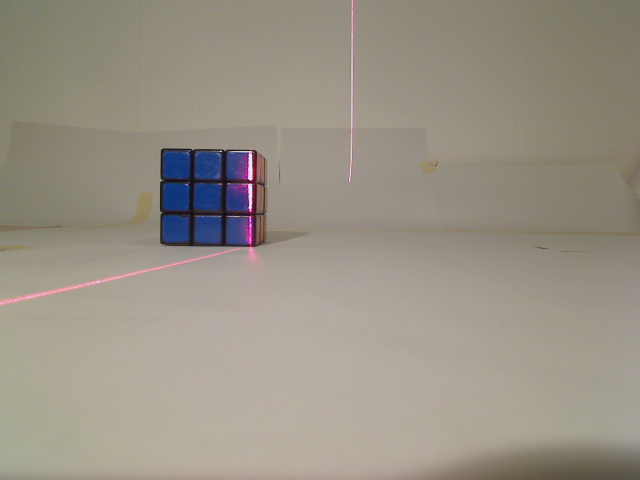
\includegraphics[width=.22\textwidth]{includes/blue_0.png}} &
		\raisebox{0.75em}{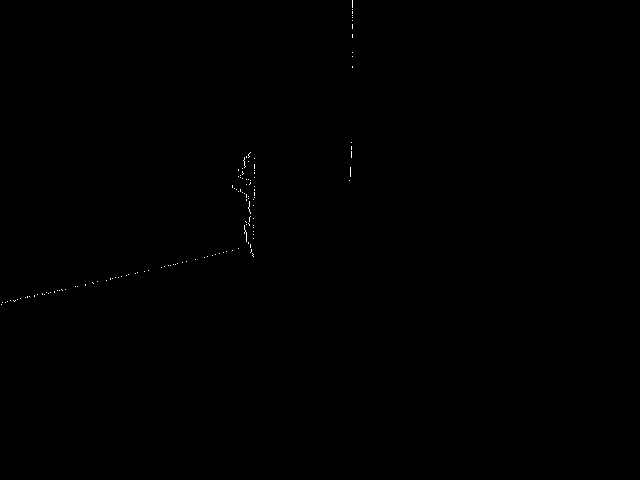
\includegraphics[width=.22\textwidth]{includes/blue_0_diff.png}} &
		\raisebox{0.75em}{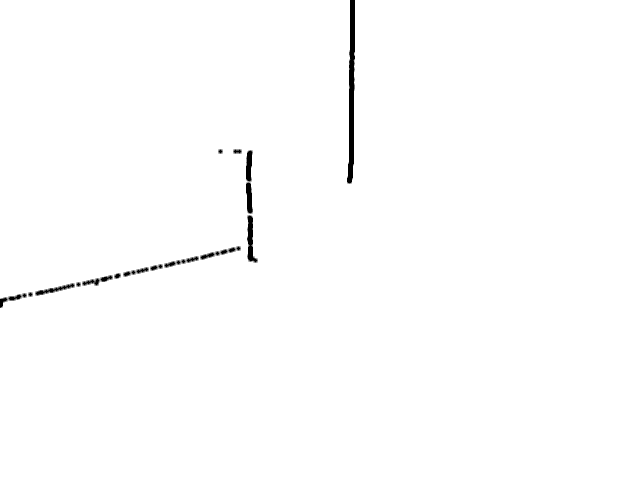
\includegraphics[width=.22\textwidth]{includes/blue_0_free.png}} &
		\raisebox{0.75em}{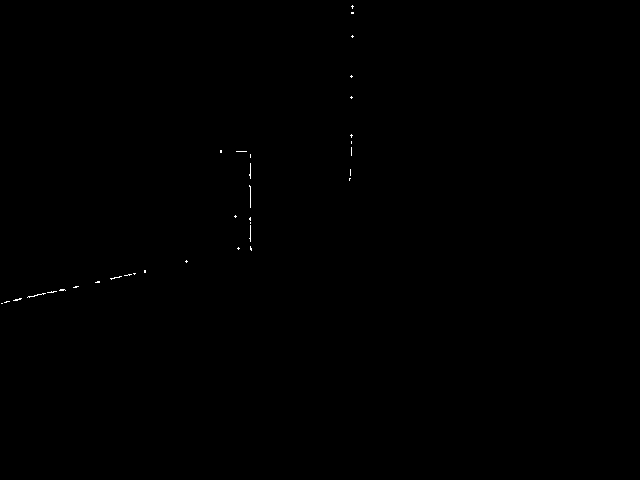
\includegraphics[width=.22\textwidth]{includes/blue_0_peak.png}} \\
		\hline
		& & \\
		\raisebox{0.75em}{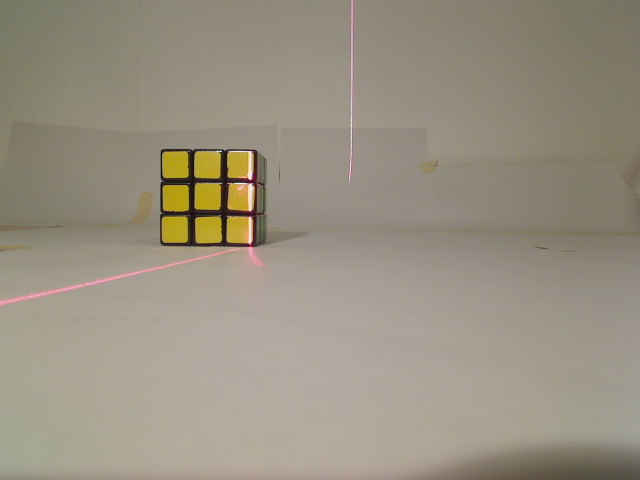
\includegraphics[width=.22\textwidth]{includes/yellow_0.png}} & 
		\raisebox{0.75em}{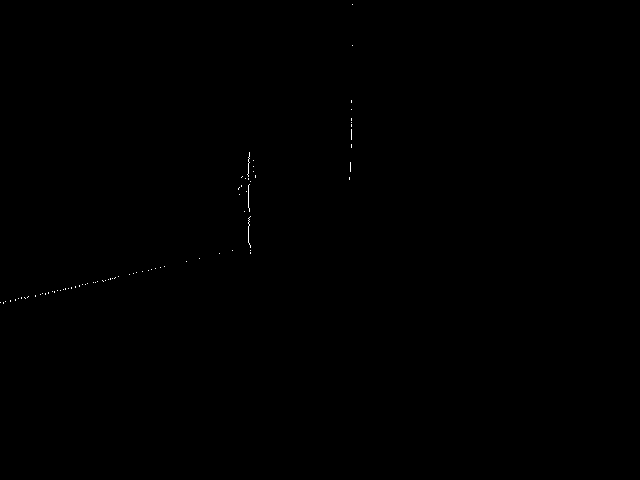
\includegraphics[width=.22\textwidth]{includes/yellow_0_diff.png}} &
		\raisebox{0.75em}{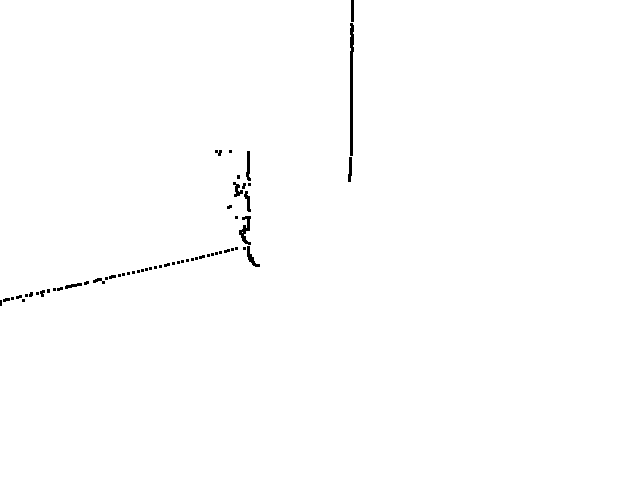
\includegraphics[width=.22\textwidth]{includes/yellow_0_free.png}} &
		\raisebox{0.75em}{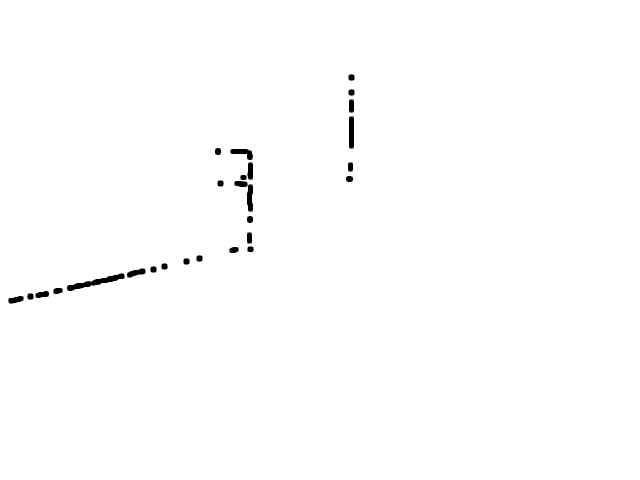
\includegraphics[width=.22\textwidth]{includes/yellow_0_peak.png}} \\
		\hline
		& & \\
		\raisebox{0.75em}{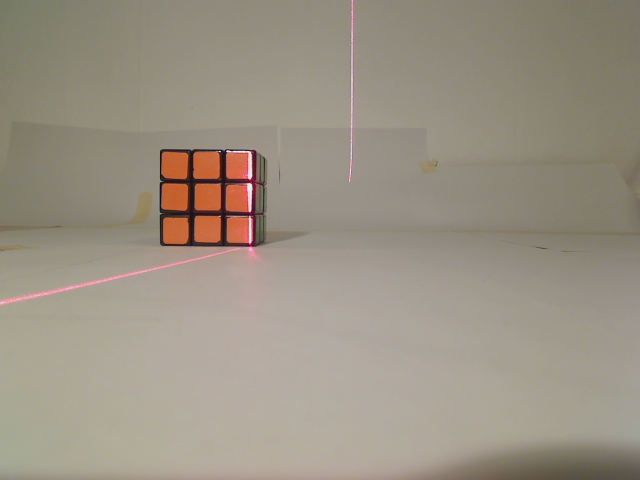
\includegraphics[width=.22\textwidth]{includes/orange_0.png}} & 
		\raisebox{0.75em}{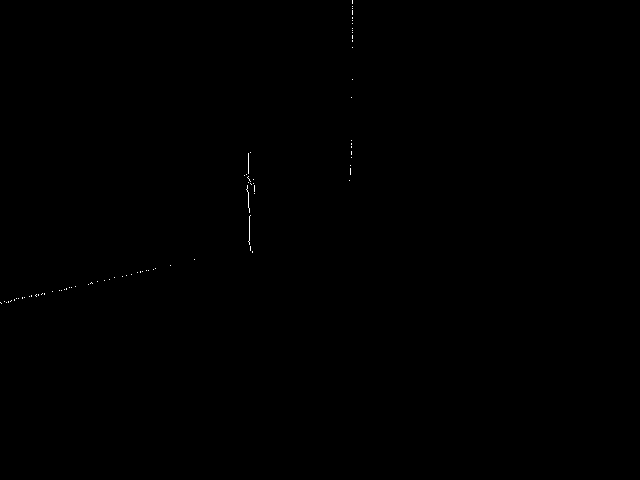
\includegraphics[width=.22\textwidth]{includes/orange_0_diff.png}} &
		\raisebox{0.75em}{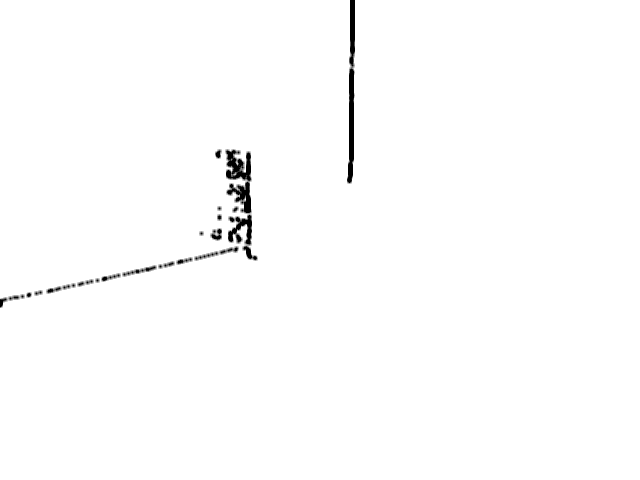
\includegraphics[width=.22\textwidth]{includes/orange_0_free.png}} &
		\raisebox{0.75em}{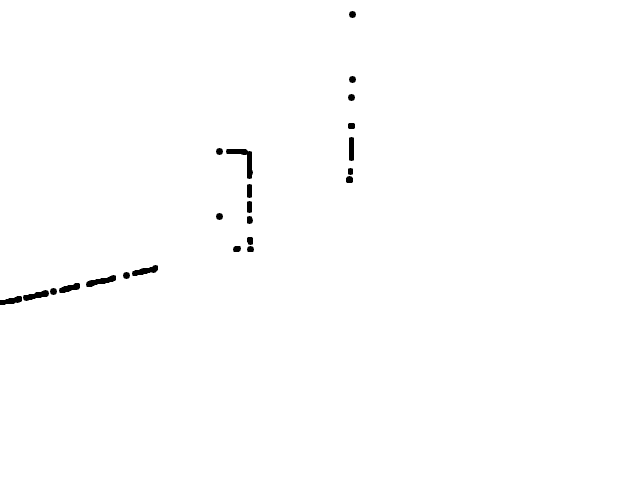
\includegraphics[width=.22\textwidth]{includes/orange_0_peak.png}}
		
	\end{tabular}
	\caption{Ergebnisse nach Diff-, Free- und Peak-Linienerkennung bei verschiedenen Farben}
	\label{fig:cols}
\end{figure}

\subsection{Verschiedene Entfernungen}
\label{sec:dists}

Als drittes wurde die blaue Seite des Würfels in verschiedenen Entfernungen vermessen, um die Entfernungsabhängigkeit der Verfahren zu bestimmen. Die Ergebnisse sind in Tabelle \ref{tab:dists}, die analog zu den vorherigen Tabellen aufgebaut ist, mit dem Unterschied, dass es eine weitere Spalte (''Diff (\%)'') gibt, in der der relative Unterschied zwischen der gemessenen und der erwarteten Entfernung steht.

Diff und Free haben bei allen Entfernungen eine relativ geringe Streuung, wohingegen Peak bei 300~mm und 400~mm Entfernung eine wesentlich höhere Streuung hat. Alle Linienerkennungen liefern ähnliche Durchschnittliche Entfernungen, wobei die gemessene Entfernung immer größer ist als die tatsächliche. Eine Ursache ist, dass die angegebene Entfernung der Abstand vom Setup zum Würfel ist, aber die Rekonstruktion die Entfernung vom Brennpunkt der Kamera zum Würfel misst. Das allein würde aber nur eine konstante Abweichung von gemessener und erwarteter Entfernung erklären, da die gemessene Entfernung aber in allen fällen 12\%-17\% größer ist und sogar mit steigender Entfernung größer wird, liegt es nahe, dass es eine weitere Fehlerquelle gibt. Ein schlecht Kalibriertes Setup ist dabei der wahrscheinlichste Kandidat.

\begin{table}[H]
	\centering
	Diff-Linienerkennung \\
	\begin{tabular}{c|c|c|c|c}
		Entfernung & Anzahl & Avg (mm) & Diff (\%) & Stdabw (mm) \\ \hline
		200 & 19048 & 224.166 & 12.0 & 8.76011 \\
		300 & 8321 & 338.722 & 12.6 & 14.8228 \\
		400 & 4294 & 460.079 & 15.0 & 14.5428 \\
		500 & 3063 & 587.986 & 17.4 & 11.6962 \\
	\end{tabular} \\
	\vspace{1em}
	Free-Linienerkennung \\
		\begin{tabular}{c|c|c|c|c}
		Entfernung & Anzahl & Avg (mm) & Diff (\%) & Stdabw (mm) \\ \hline
		200 & 5733 & 225.367 & 12.5 & 1.08721 \\
		300 & 3535 & 340.892 & 13.3 & 2.82819 \\
		400 & 1475 & 461.271 & 15.3 & 3.90112 \\
		500 & 1156 & 586.405 & 17.2 & 7.37468 \\
	\end{tabular} \\
	\vspace{1em}
	Peak-Linienerkennung \\
		\begin{tabular}{c|c|c|c|c}
		Entfernung & Anzahl & Avg (mm) & Diff (\%) & Stdabw (mm) \\ \hline
		200 & 7272 & 226.148 & 13.0 & 21.1726 \\
		300 & 6543 & 341.249 & 13.7 & 234.736 \\
		400 & 1849 & 462.031 & 15.5 & 163.782 \\
		500 & 1200 & 586.895 & 17.2 & 34.1902 \\
	\end{tabular} \\
	\caption{Scans der blauen Seiten in verschiedenen Entfernungen}
	\label{tab:dists}
\end{table}

\subsection{Verschiedene Beleuchtungen}

Zuletzt wurden die Einflüsse unterschiedlicher Beleuchtungen untersucht. Bisher wurde der ''Rubik's Cube'' direkt von einer Schreibtischlampe und von einer Deckenlampe beleuchtet. Nun wurde einmal die Schreibtischlampe und einmal die Deckenbeleuchtung ausgeschaltet. Der Versuch konnte nicht bei vollständiger Dunkelheit durchgeführt werden, da dabei das Referenzbild komplett schwarz wäre, was es unmöglich macht zu unterscheiden, ob ein Messpunkt zur Würfeloberfläche gehört oder nicht. Die Ergebnisse sind in Tabelle \ref{tab:lights} zu sehen.

Wie bereits in Abschnitt \ref{sec:reps} angesprochen, spiegelt sich der Laser im Würfel, was, wie man in den Abbildung \ref{fig:lights} sehen kann, von der Diff-Linienerkennung fälschlicherweise als Linie erkannt wird. Bei schwächerer Beleuchtung ist der Spiegeleffekt stärker, was dazu führt, dass Diff bei der Beleuchtung nur durch die Deckenlampe schlechtere Ergebnisse liefert, als bei einer direkten Beleuchtung durch die Schreibtischlampe. Beide Lampen zusammen liefern die besten Ergebnisse.

Die Free-Linienerkennung wird durch diese Spiegeleffekte nicht beeinflusst, allerdings erkennt sie, wie man in Abbildung \ref{fig:lights} sehen kann, falsche Punkte auf dem Boden. Die Beleuchtung durch die Schreibtischlampe sorgt dafür, dass es hellere und dunklere Bereiche in dem Bild gibt. Das führt dazu, dass wie in Abschnitt \ref{sec:cols} der Mittelwert verzerrt wird und auch falsche Punkte erkannt werden.

Die Peak-Linienerkennung liefert schlechtere Ergebnisse wenn die Szene heller Beleuchtet ist. Das liegt daran, dass bei einem dunkleren Hintergrund der Unterschied zwischen dem blauen Würfel und der Wand kleiner ist und dadurch weniger falsche Punkte an der Kante des Würfels erkannt werden.

\begin{table}[H]
	\centering
	Diff-Linienerkennung \\
	\begin{tabular}{c|c|c|c}
		Beleuchtung & Anzahl & Avg (mm) & Stdabw (mm) \\ \hline
		Schreibtischlampe & 9264 & 338.236 & 34.9526 \\
		Deckenlampe & 12267 & 335.573 & 97.8706 \\
		Schreibtisch- und Deckenlampe & 8321 & 338.722 & 14.8228 \\
	\end{tabular} \\
	\vspace{1em}
	Free-Linienerkennung \\
		\begin{tabular}{c|c|c|c}
		Beleuchtung & Anzahl & Avg (mm) & Stdabw (mm) \\ \hline
		Schreibtischlampe & 4451 & 340.415 & 32.2099 \\
		Deckenlampe & 5890 & 339.616 & 2.99821 \\
		Schreibtisch- und Deckenlampe & 3535 & 340.892 & 2.82819 \\
	\end{tabular} \\
	\vspace{1em}
	Peak-Linienerkennung \\
		\begin{tabular}{c|c|c|c}
		Beleuchtung & Anzahl & Avg (mm) & Stdabw (mm) \\ \hline
		Schreibtischlampe & 7144 & 340.854 & 159.129 \\
		Deckenlampe & 6108 & 340.663 & 9.15014 \\
		Schreibtisch- und Deckenlampe & 6543 & 341.249 & 234.736 \\
	\end{tabular} \\
	\caption{Scans der blauen Seiten in 300~mm Entfernungen mit verschiedenen Beleuchtungen}
	\label{tab:lights}
\end{table}


\begin{figure}[H]
	\centering
	
	\begin{tabular}{c|c|c|c}
		& Schreibtischlampe & Deckenlampe & beide Lampen \\
		\hline
		 & & & \\
		\rotatebox{90}{\hspace{3em} Kamera} &
		\raisebox{0.75em}{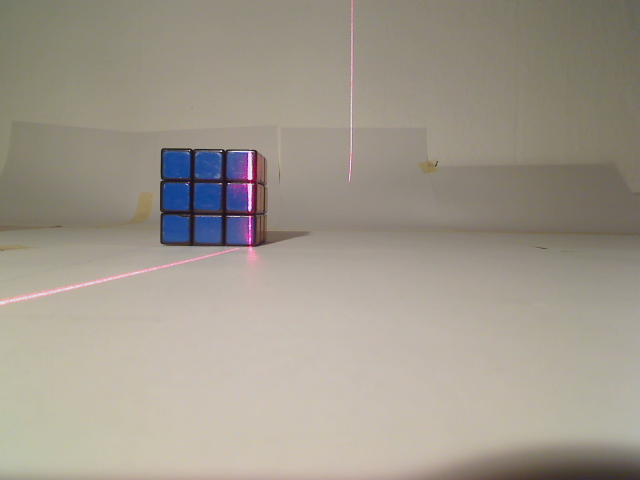
\includegraphics[width=.3\textwidth]{includes/blue_d.png}} & 
		\raisebox{0.75em}{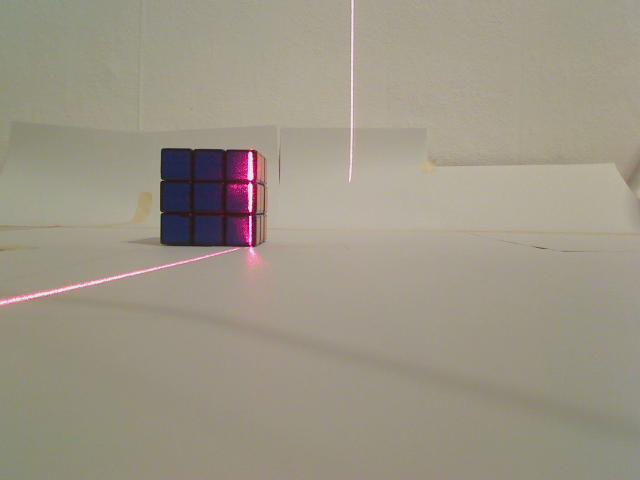
\includegraphics[width=.3\textwidth]{includes/blue_t.png}} &
		\raisebox{0.75em}{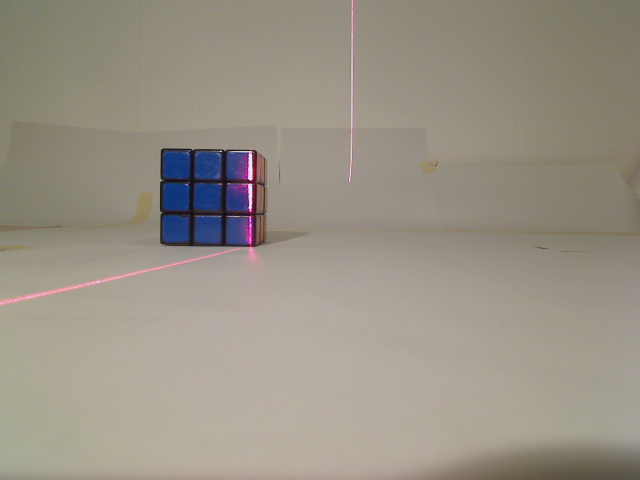
\includegraphics[width=.3\textwidth]{includes/blue_dt.png}} \\
		\hline
		& & \\
		\rotatebox{90}{\hspace{4em} Diff} &
		\raisebox{0.75em}{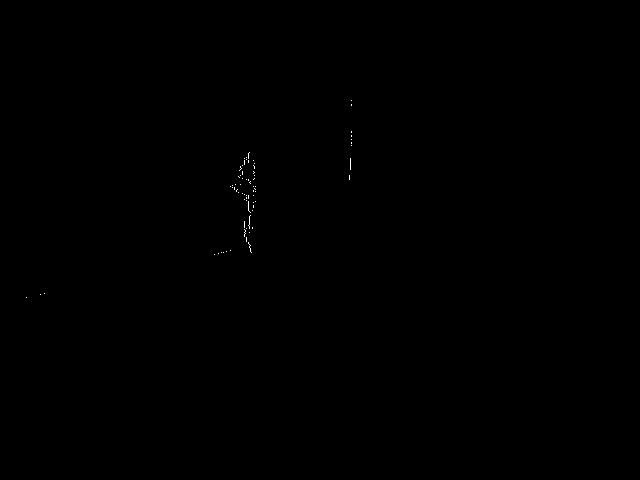
\includegraphics[width=.3\textwidth]{includes/blue_d_diff.png}} & 
		\raisebox{0.75em}{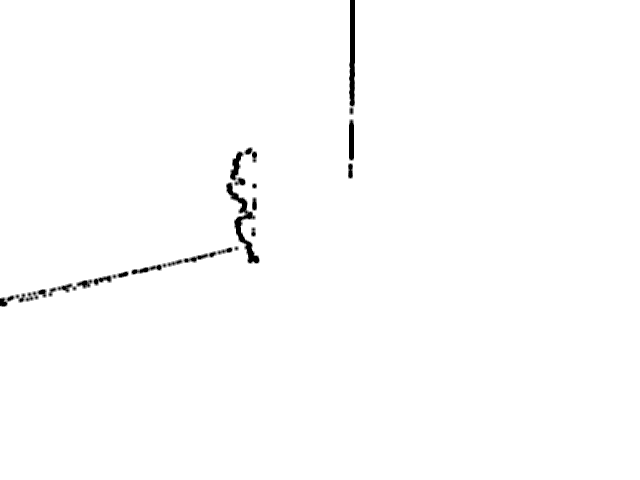
\includegraphics[width=.3\textwidth]{includes/blue_t_diff.png}} &
		\raisebox{0.75em}{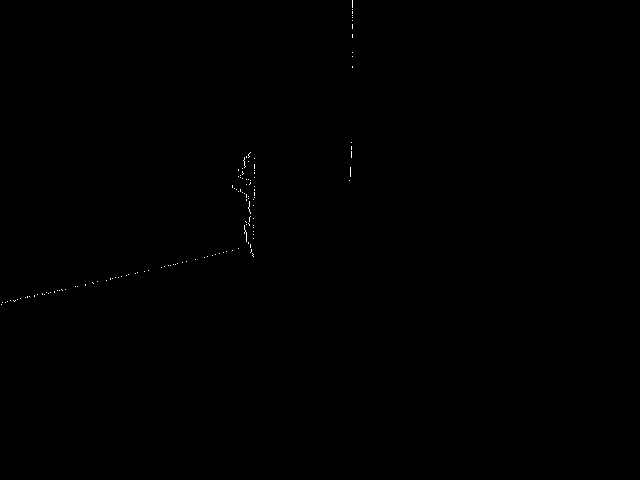
\includegraphics[width=.3\textwidth]{includes/blue_dt_diff.png}} \\
		\hline
		& & \\
		\rotatebox{90}{\hspace{4em} Free} &
		\raisebox{0.75em}{\includegraphics[width=.3\textwidth]{includes/blue_d_free.png}} & 
		\raisebox{0.75em}{\includegraphics[width=.3\textwidth]{includes/blue_t_free.png}} &
		\raisebox{0.75em}{\includegraphics[width=.3\textwidth]{includes/blue_dt_free.png}} \\
		\hline
		& & \\
		\rotatebox{90}{\hspace{4em} Peak} &
		\raisebox{0.75em}{\includegraphics[width=.3\textwidth]{includes/blue_d_peak.png}} & 
		\raisebox{0.75em}{\includegraphics[width=.3\textwidth]{includes/blue_t_peak.png}} &
		\raisebox{0.75em}{\includegraphics[width=.3\textwidth]{includes/blue_dt_peak.png}}
		
	\end{tabular}
	\caption{Ergebnisse nach Diff-, Free- und Peak-Linienerkennung bei verschiedenen Beleuchtungen}
	\label{fig:lights}
\end{figure}


% ---------------------------------------------------------------------------- %

\section{Zusammenfassung}
\label{sec:summary}

Es gibt viele Möglichkeiten ein Objekt zu vermessen.
In unserem Semesterprojekt haben wir uns mit der Streifenlichtprojektion beschäftigt, eine Umsetzung entworfen und deren Ergebnisse ausgewertet.
Wir steuern mit Hilfe eines Mikrocontrollers einen Streifenlaser an, mit dem wir eine Linie in die Szene projizieren.
Mit einer einfachen Webcam nehmen wir die Szene auf und geben die Aufnahmen an die Verarbeitungssoftware weiter.
Deren erster Schritt ist es die Linie in der Aufnahme zu finden.
Für diesem Zweck wurden mehrere Ansätze implementiert.

Ein Ansatz berechnet die Differenz zwischen der Aufnahme und einem Referenzbild (Diff), während ein anderer mit Hilfe von Mittelwerten über dem gesamten Bild (Free) oder Mittelwerten lediglich in einer kleineren Umgebung eines Pixels (Peak) arbeitet.
Das Ergebnis der Linienerkennung ist ein Binärbild, aus dem die Punkte der Linie direkt bestimmt werden können.

Aus den Positionen im Bild kann als nächstes die Entfernung der Objektpunkte berechnet werden.
Dazu werden mit Hilfe bekannter Größen aus dem Setup und der Triangulation die 3-D-Koordinaten für jeden Punkt der Linie berechnet.

Um die verschiedenen Ansätze vergleichen zu können und Grenzen dieses Verfahrens und seiner Umsetzung ausloten zu können, wurden verschiedene Testreihen durchgeführt.
Dazu wurde ein Rubiks-Cube von verschiedenen Seiten unter verschiedenen Bedingungen aufgenommen und die Ergebnisse verglichen.
Die Ergebnisse zeigen, dass die Diff-Linienerkennung Probleme mit spiegelnden Oberflächen hat.
Diese Effekte können mit verschiedenen Beleuchtungen der Szene verstärkt/abgeschwächt werden.
Mit der roten Oberfläche kommen beide Ansätze relativ gut zurecht, während beide mit der gelben Oberfläche ähnlich schlechte Ergebnisse liefern.
Bei Tests mit anderen Farben unterscheiden sich die Ansätze zum Teil sehr stark.
Alles in allem lässt sich aus den Tests entnehmen, dass die Diff-Linienerkennung weniger zwischen unterschiedlichen Farben schwankt als die Free-Linienerkennung.

Zusammenfassend kann man sagen, dass unsere Umsetzung der Messmethode Streifenlichtprojektion für die investierten Ressourcen ziemlich gute Ergebnisse liefert und dabei mit herkömmlichem Equipment auskommt.
Um die Ergebnisse weiter zu verbessern schlagen wir vor ein präziseres Setup zu verwenden, das genauer vermessen werden kann und resistenter gegenüber physische Störungen ist. In vielen Fällen würde eine robustere Linienerkennung ebenfalls für deutlich bessere Ergebnisse sorgen.

% ---------------------------------------------------------------------------- %

\section{Quellenverzeichnis}

% ---------------------------------------------------------------------------- %

\end{document}
